
\section{Results}

\subsection{Displacement and velocity amplitude}

The displacement amplitude as a function of $U^*$ (Fig.\ref{fig:QSS_FSI_dis_amp}) shows a shift in the curves when the damping ratio is increased. This phenomenon could be observed in the velocity amplitude curves as well(Fig. \ref{fig:QSS_FSI_vel_amp}).

\subsection{Mean power}

The influence of $m^*$ and $\zeta$ on mean power obtained using Eq.\ref{power}  was investigated separately. Two data sets were obtained by keeping each variable constant and changing the other  Fig. \ref{fig:power_barrero_style_zeta_165} and \ref{fig:power_barrero_style_mstar_165}. The mean power curves at obtained by varying $\zeta$ shows a shift to the right (Fig.\ref{fig:power_barrero_style_zeta_165}) as $\zeta$ was increased. However, the maximum mean power remains constant.  The shift of curves was also observed when the $m^*$ varied. A similar kind of behaviour was observed by \cite{Barrero-Gil2010a} where he concluded that the maximum power attainable efficiency does not depend on $m^*\zeta$ parameter. However, at $m^* \leq 30$ an effect of $m^*$ could be observed, where the maximum of the mean power curve reduced as $m^*$ was reduced.

\begin{figure}
\centering
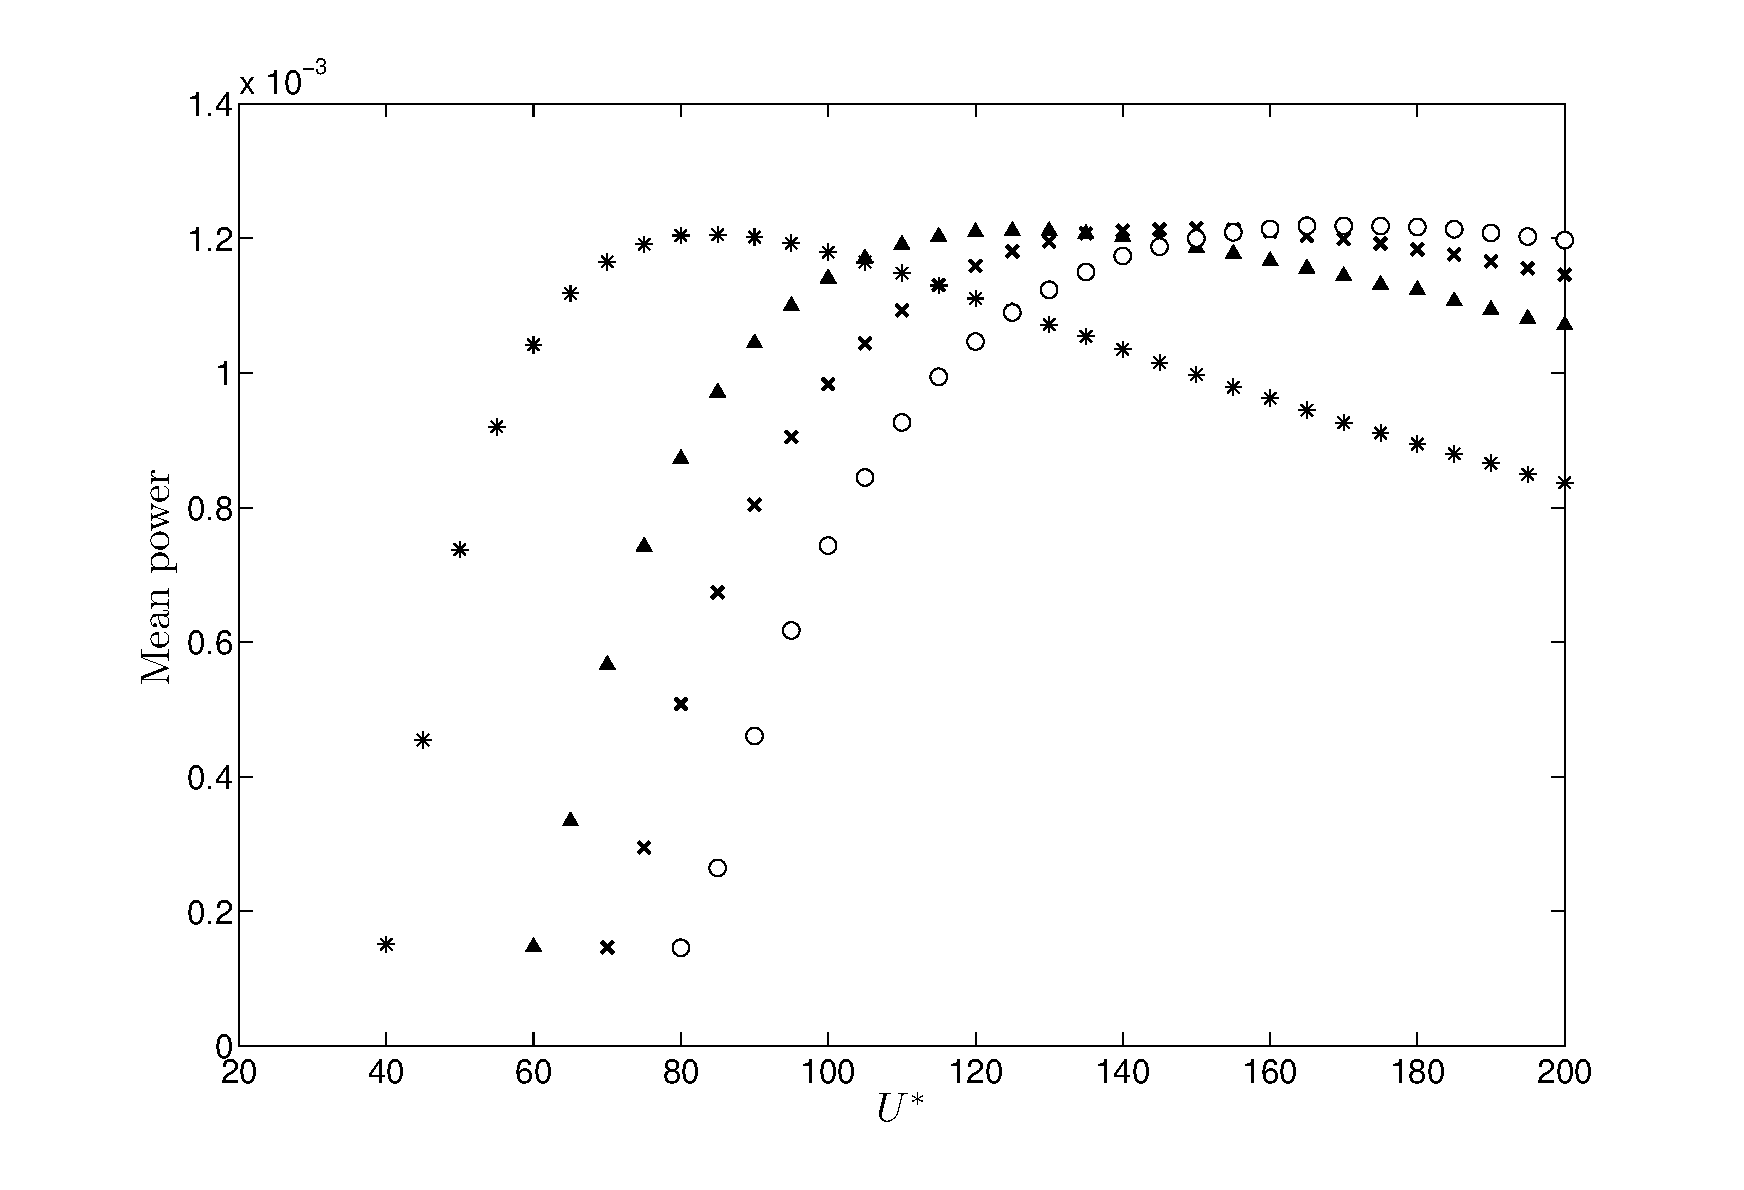
\includegraphics[width=0.8\linewidth]{../FnP/power_barrero_style_zeta_165}
\caption{}
\label{fig:power_barrero_style_zeta_165}
\end{figure}


\begin{figure}
\centering
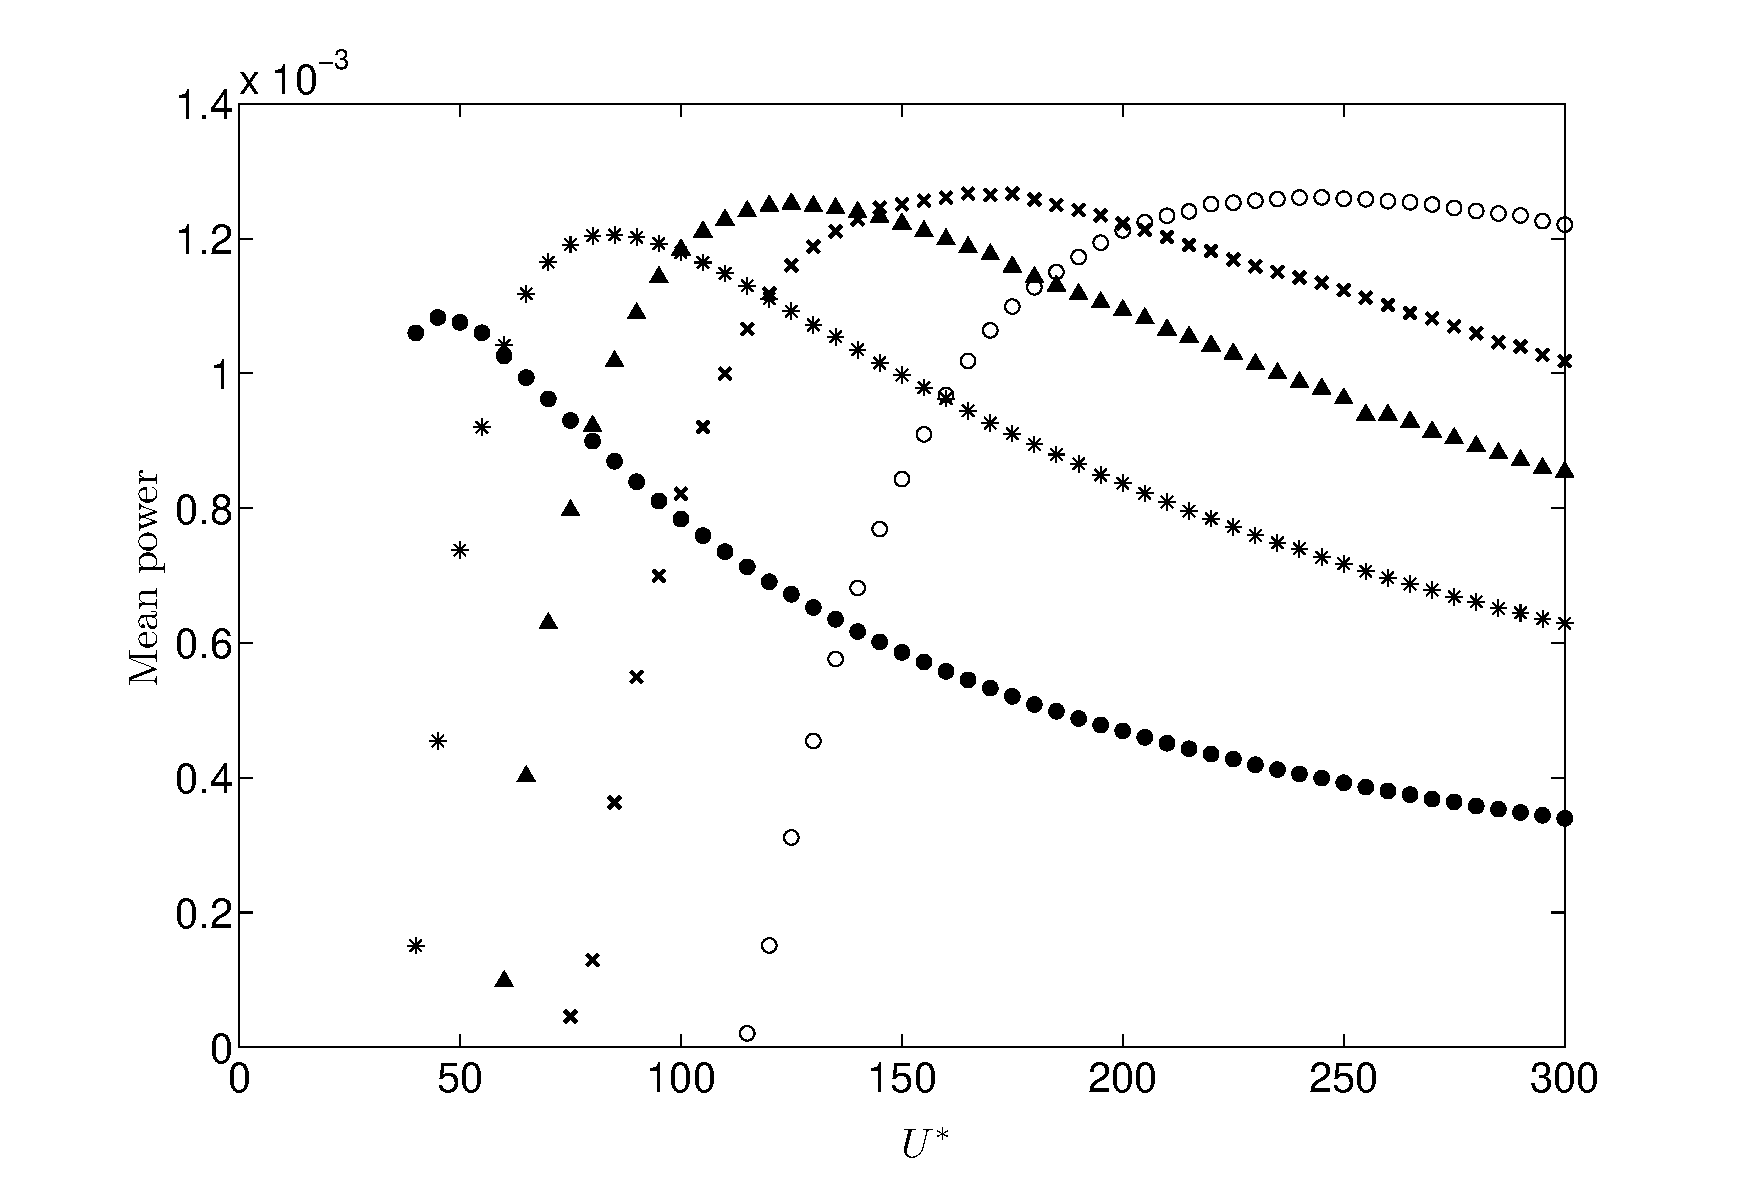
\includegraphics[width=0.8\linewidth]{../FnP/power_barrero_style_mstar_165}
\caption{}
\label{fig:power_barrero_style_mstar_165}
\end{figure}


\hilight{Put parkinson data }
The data obtained using $C_y$ data from \cite{Parkinson1964} shows the same trend (\ref{fig:mean_power_park}) where a shift to the right of the peak power could be observed with increasing $\zeta$. Hysteresis was also present in the mean power data, which was achieved by changing the initial conditions of the system.


\begin{figure}
\centering
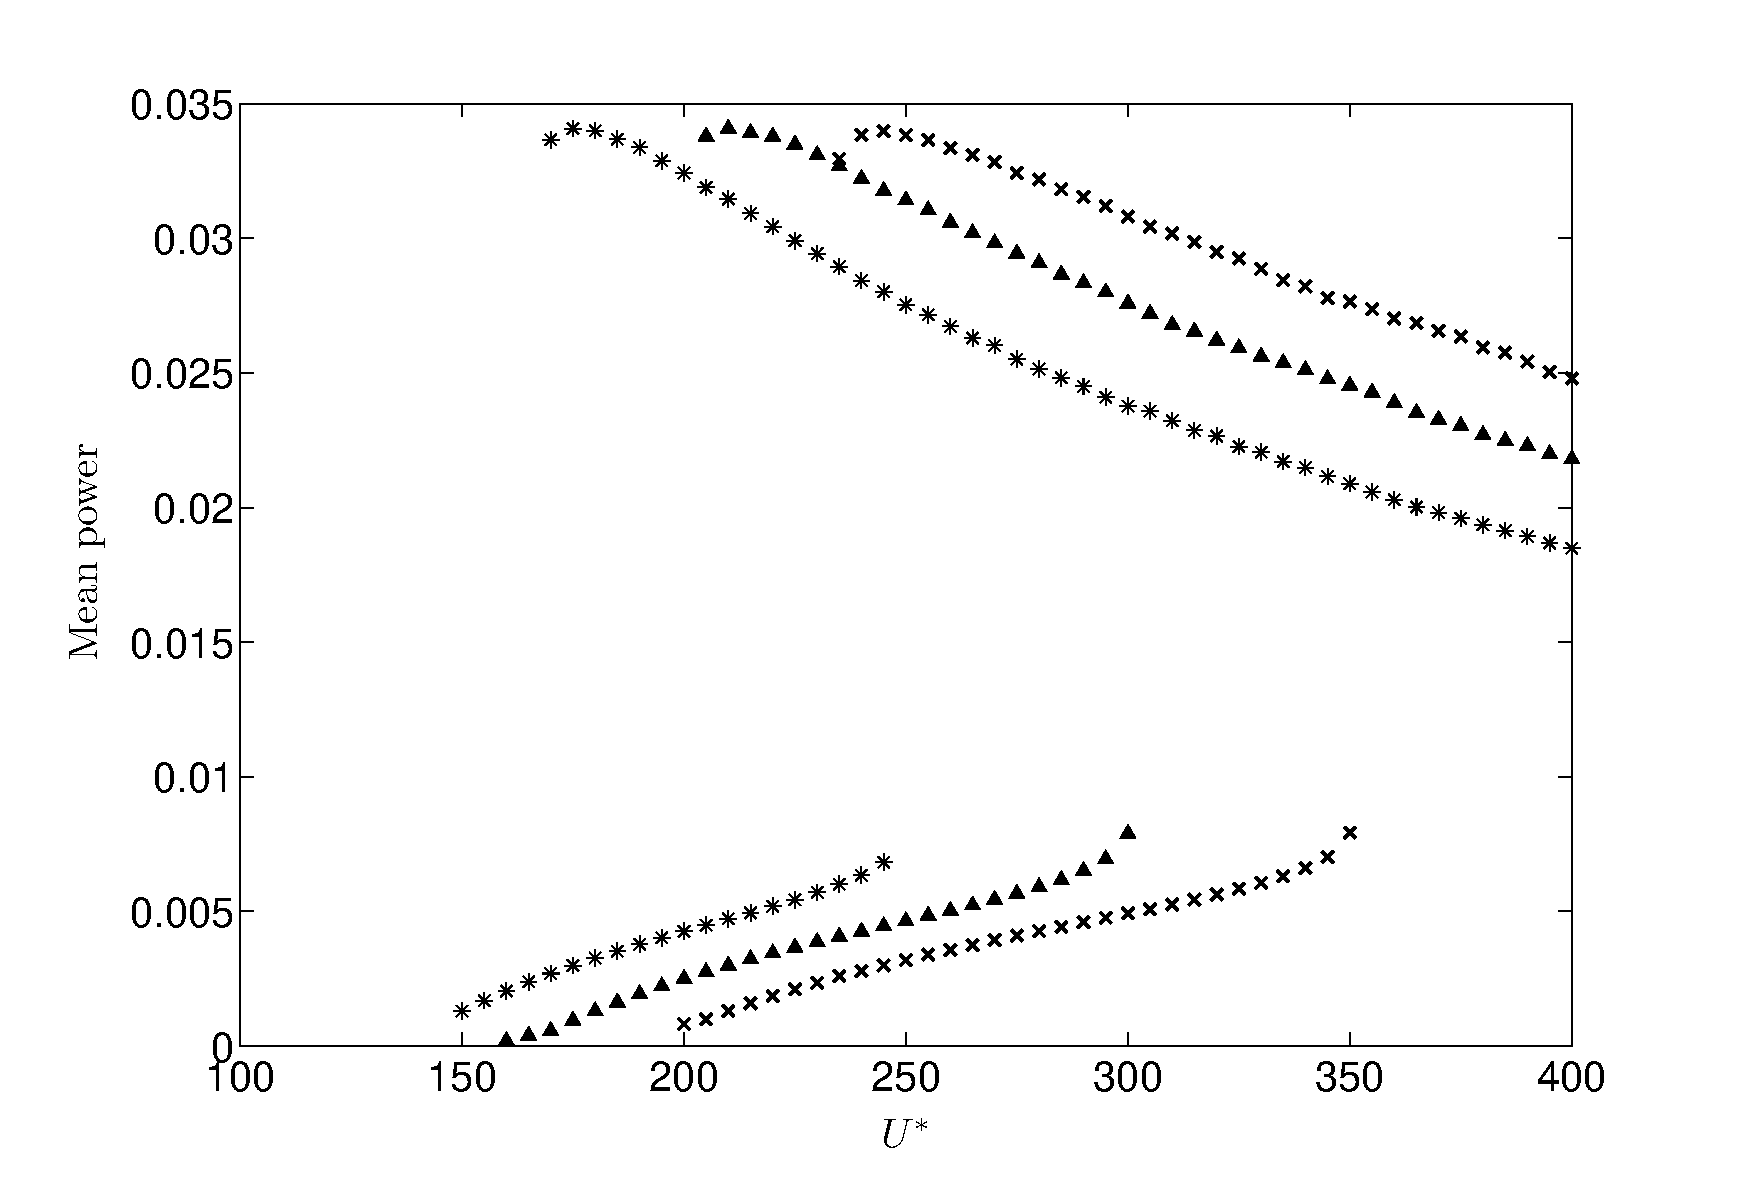
\includegraphics[width=0.8\linewidth]{../FnP/from_reynolds/mean_power_park}
\caption{}
\label{fig:mean_power_park}
\end{figure}




The most interesting fact was that the data ( displacement amplitude, velocity amplitude and mean power) could be collapsed regardless of $m^*$ or $\zeta$ when it was plot against the damping constant i.e. `$c$'.

\begin{figure}
\centering
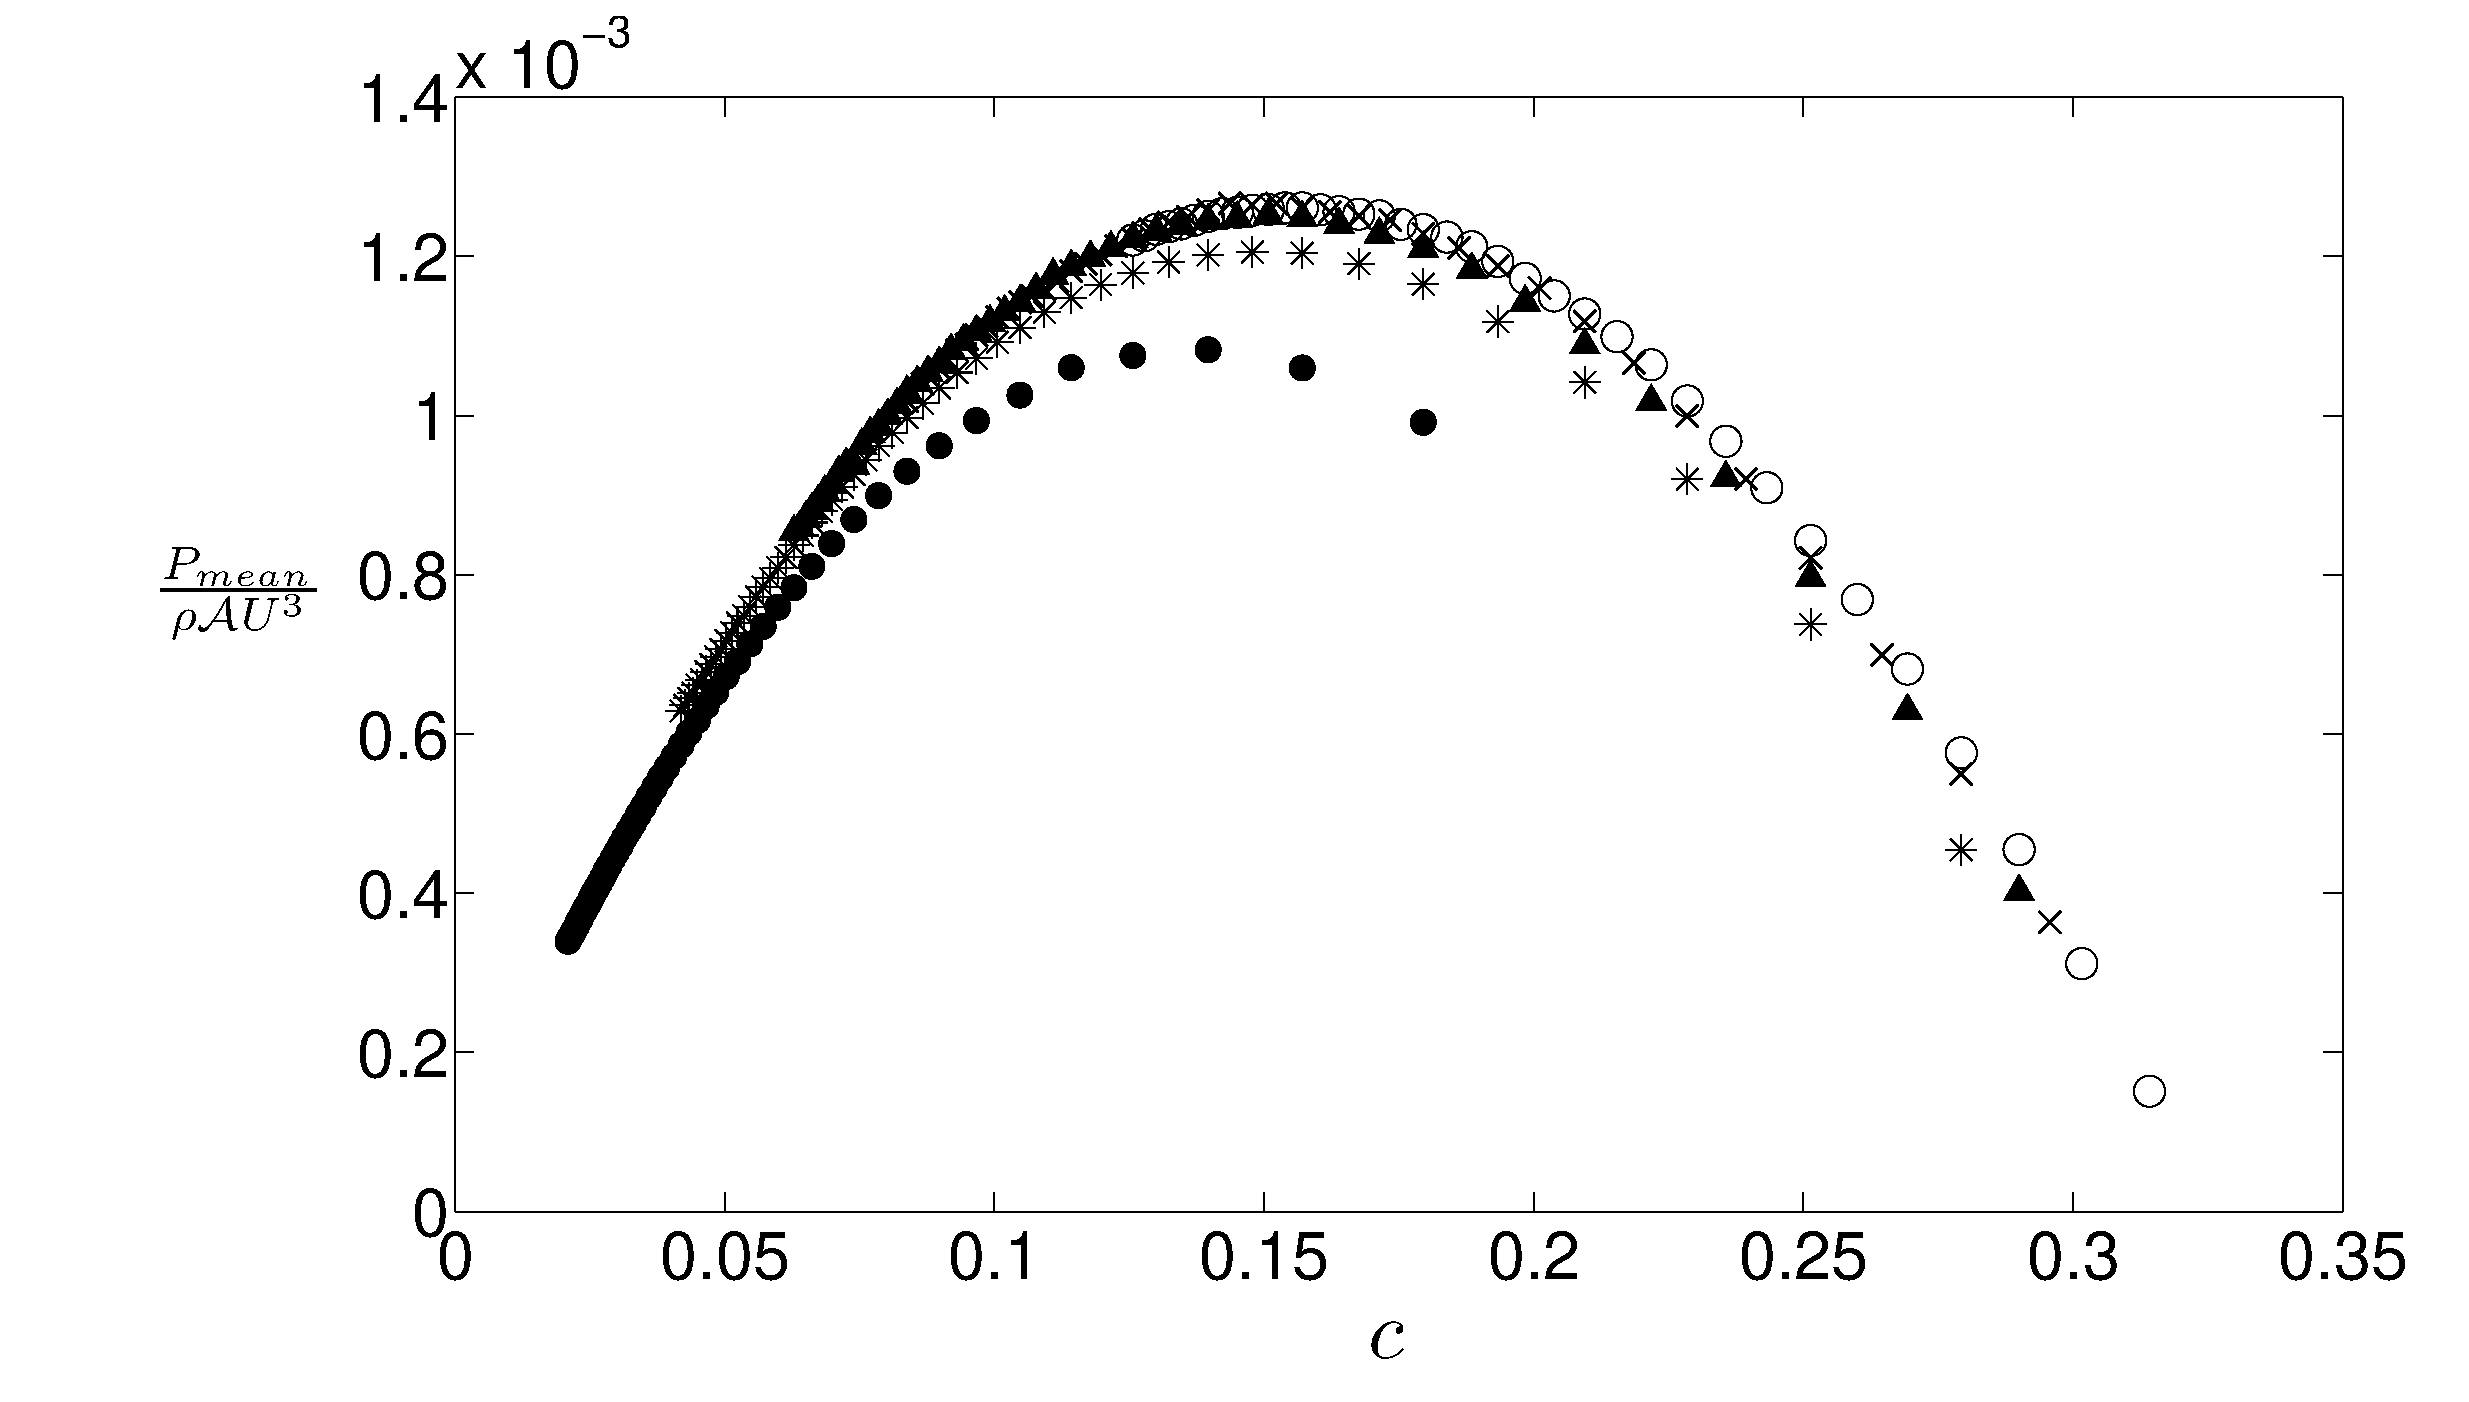
\includegraphics[width=0.8\linewidth]{../FnP/power_barrero_style_mstar_collapsed_165}
\caption{Mean power vs. damping ratio at different $m^*$ $\zeta=0.1$ (,\ding{108} $m^*=10$,\ding{83} $m^*=20$, \ding{115} $m^*=30$, $\times$ $m^*=40$ and  $\bigcirc$ $m^* = 60$, at Re = 165) } 
\label{fig:power_barrero_style_mstar_collapsed_165}
\end{figure}


\begin{figure}
\centering
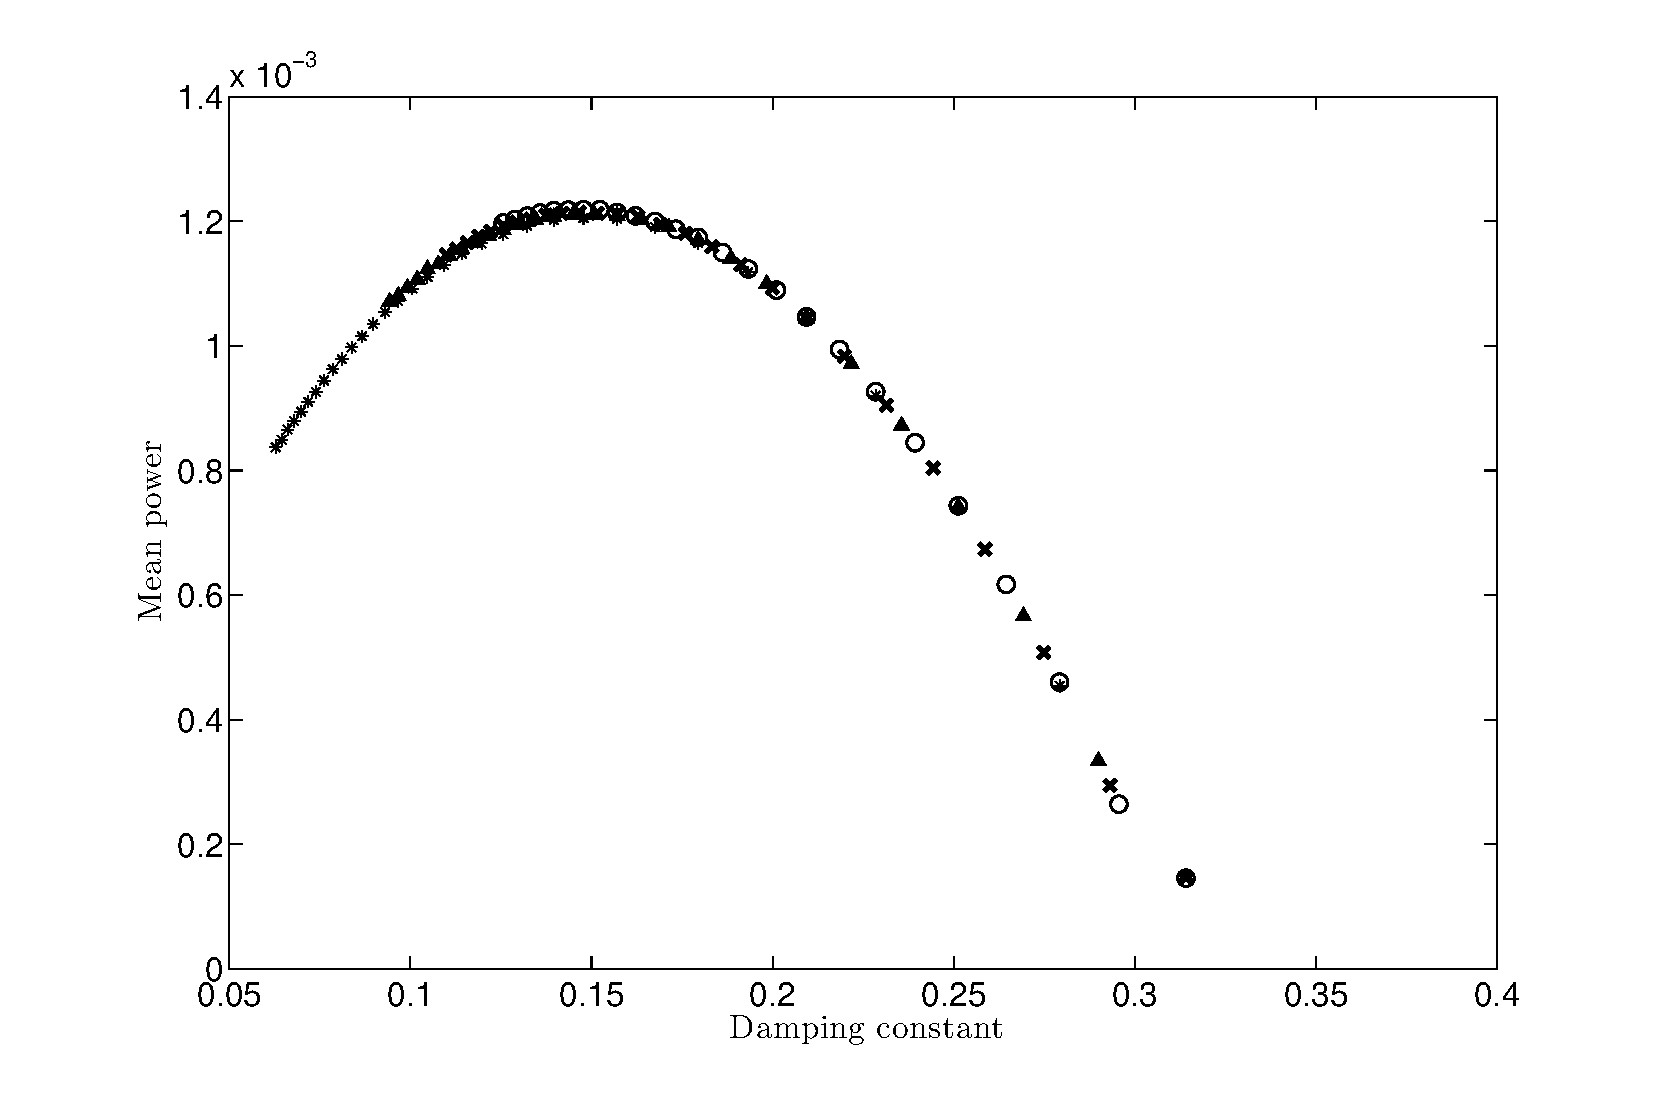
\includegraphics[width=0.8\linewidth]{../FnP/power_barrero_style_cstar_collapsed_165}
\caption{Mean power vs. damping constant at $m^*=20$. \ding{83} $ \zeta = 0.1$, \ding{115} $\zeta = 0.15$,   $\times$ $\zeta = 0.175$ and $\circ$ $\zeta = 0.2$}
\label{fig:power_barrero_style_cstar_collapsed_165}
\end{figure}


\begin{figure}
\centering
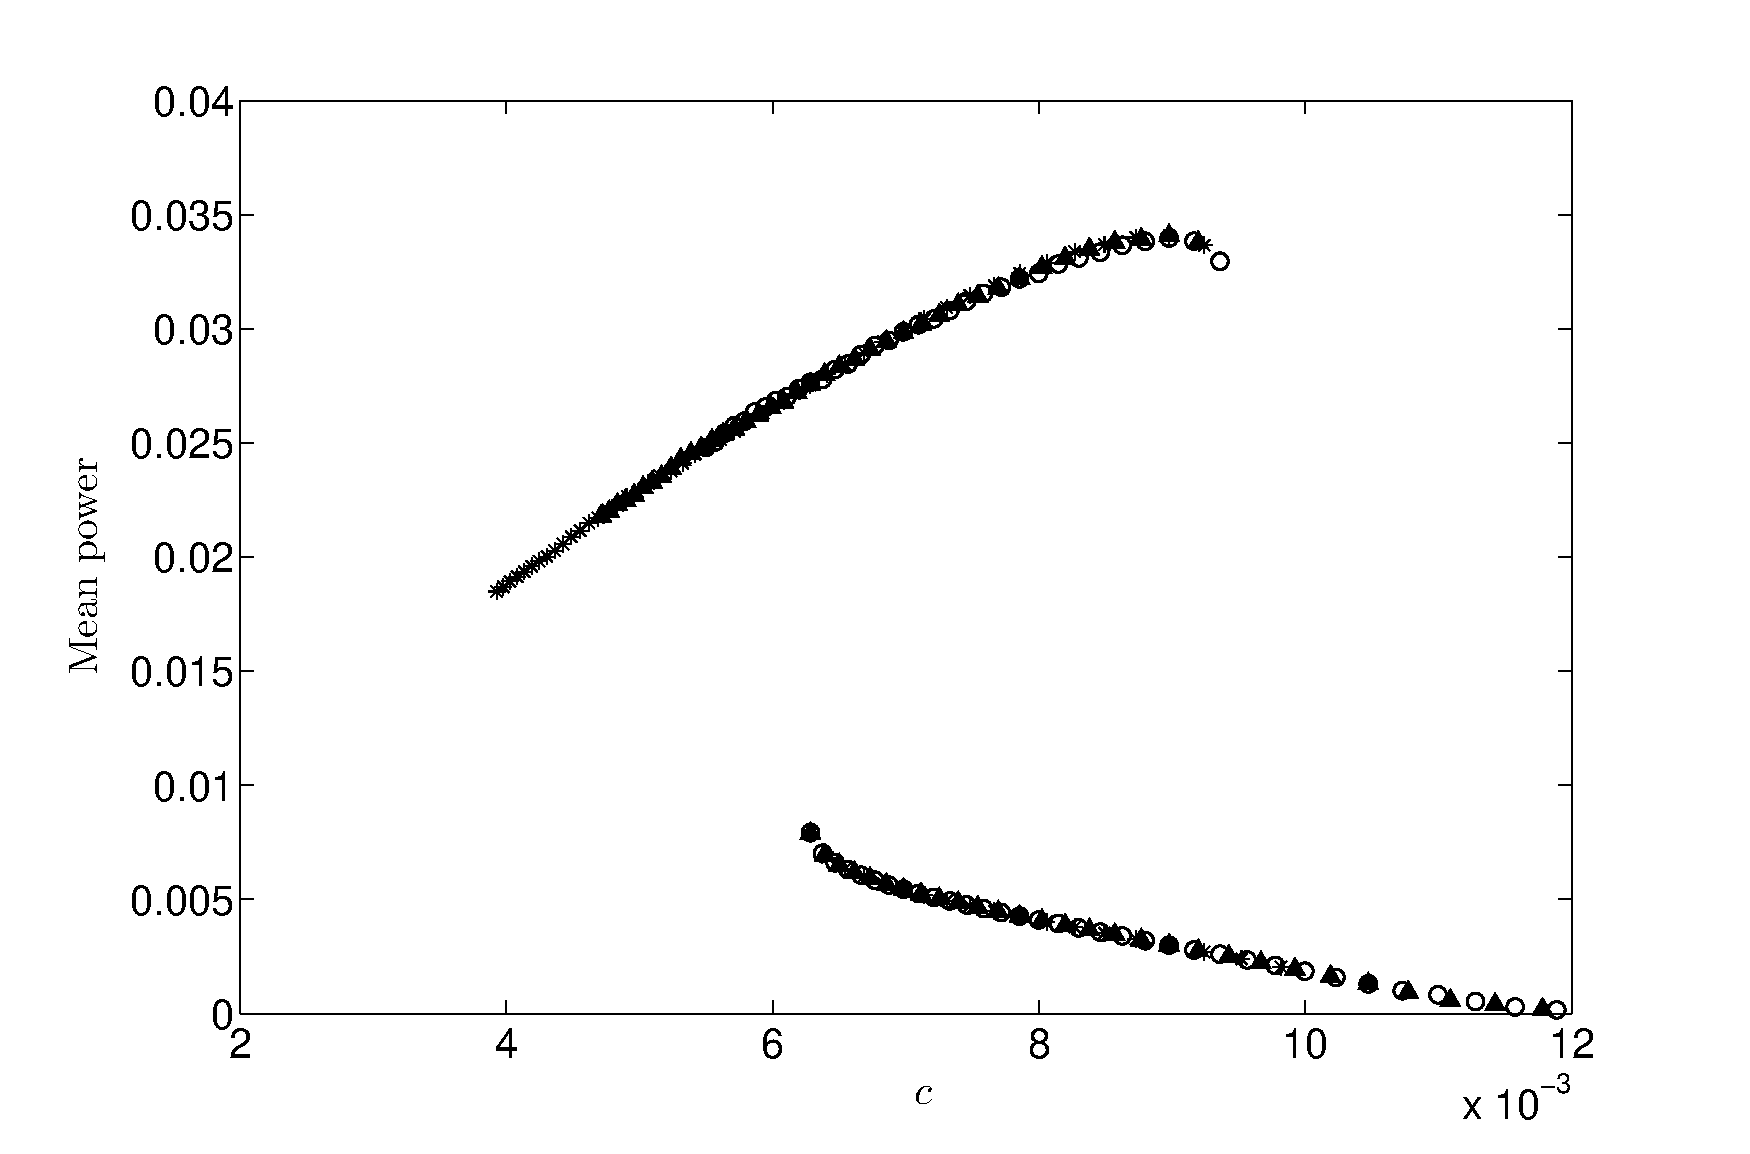
\includegraphics[width=0.8\linewidth]{../FnP/from_reynolds/mean_power_park_collapsed}
\caption{}
\label{fig:mean_power_park_collapsed}
\end{figure}




\subsection{Comparison of FSI and QSS data at Re-165}

The displacement and velocity amplitude shows similar trends between FSI and QSS simulations (Fig. \ref{fig:QSS_FSI_dis_amp} and \ref{fig:QSS_FSI_vel_amp}.). Quantitatively a large discrepancy  could be observed between QSS and FSI data. The cause for this would be  due to the damping caused by the fluid (due to viscous effects or fluid drag when the body moves transversely). At low Reynolds numbers viscous effects are more prominent.

%\begin{figure}
%\centering
%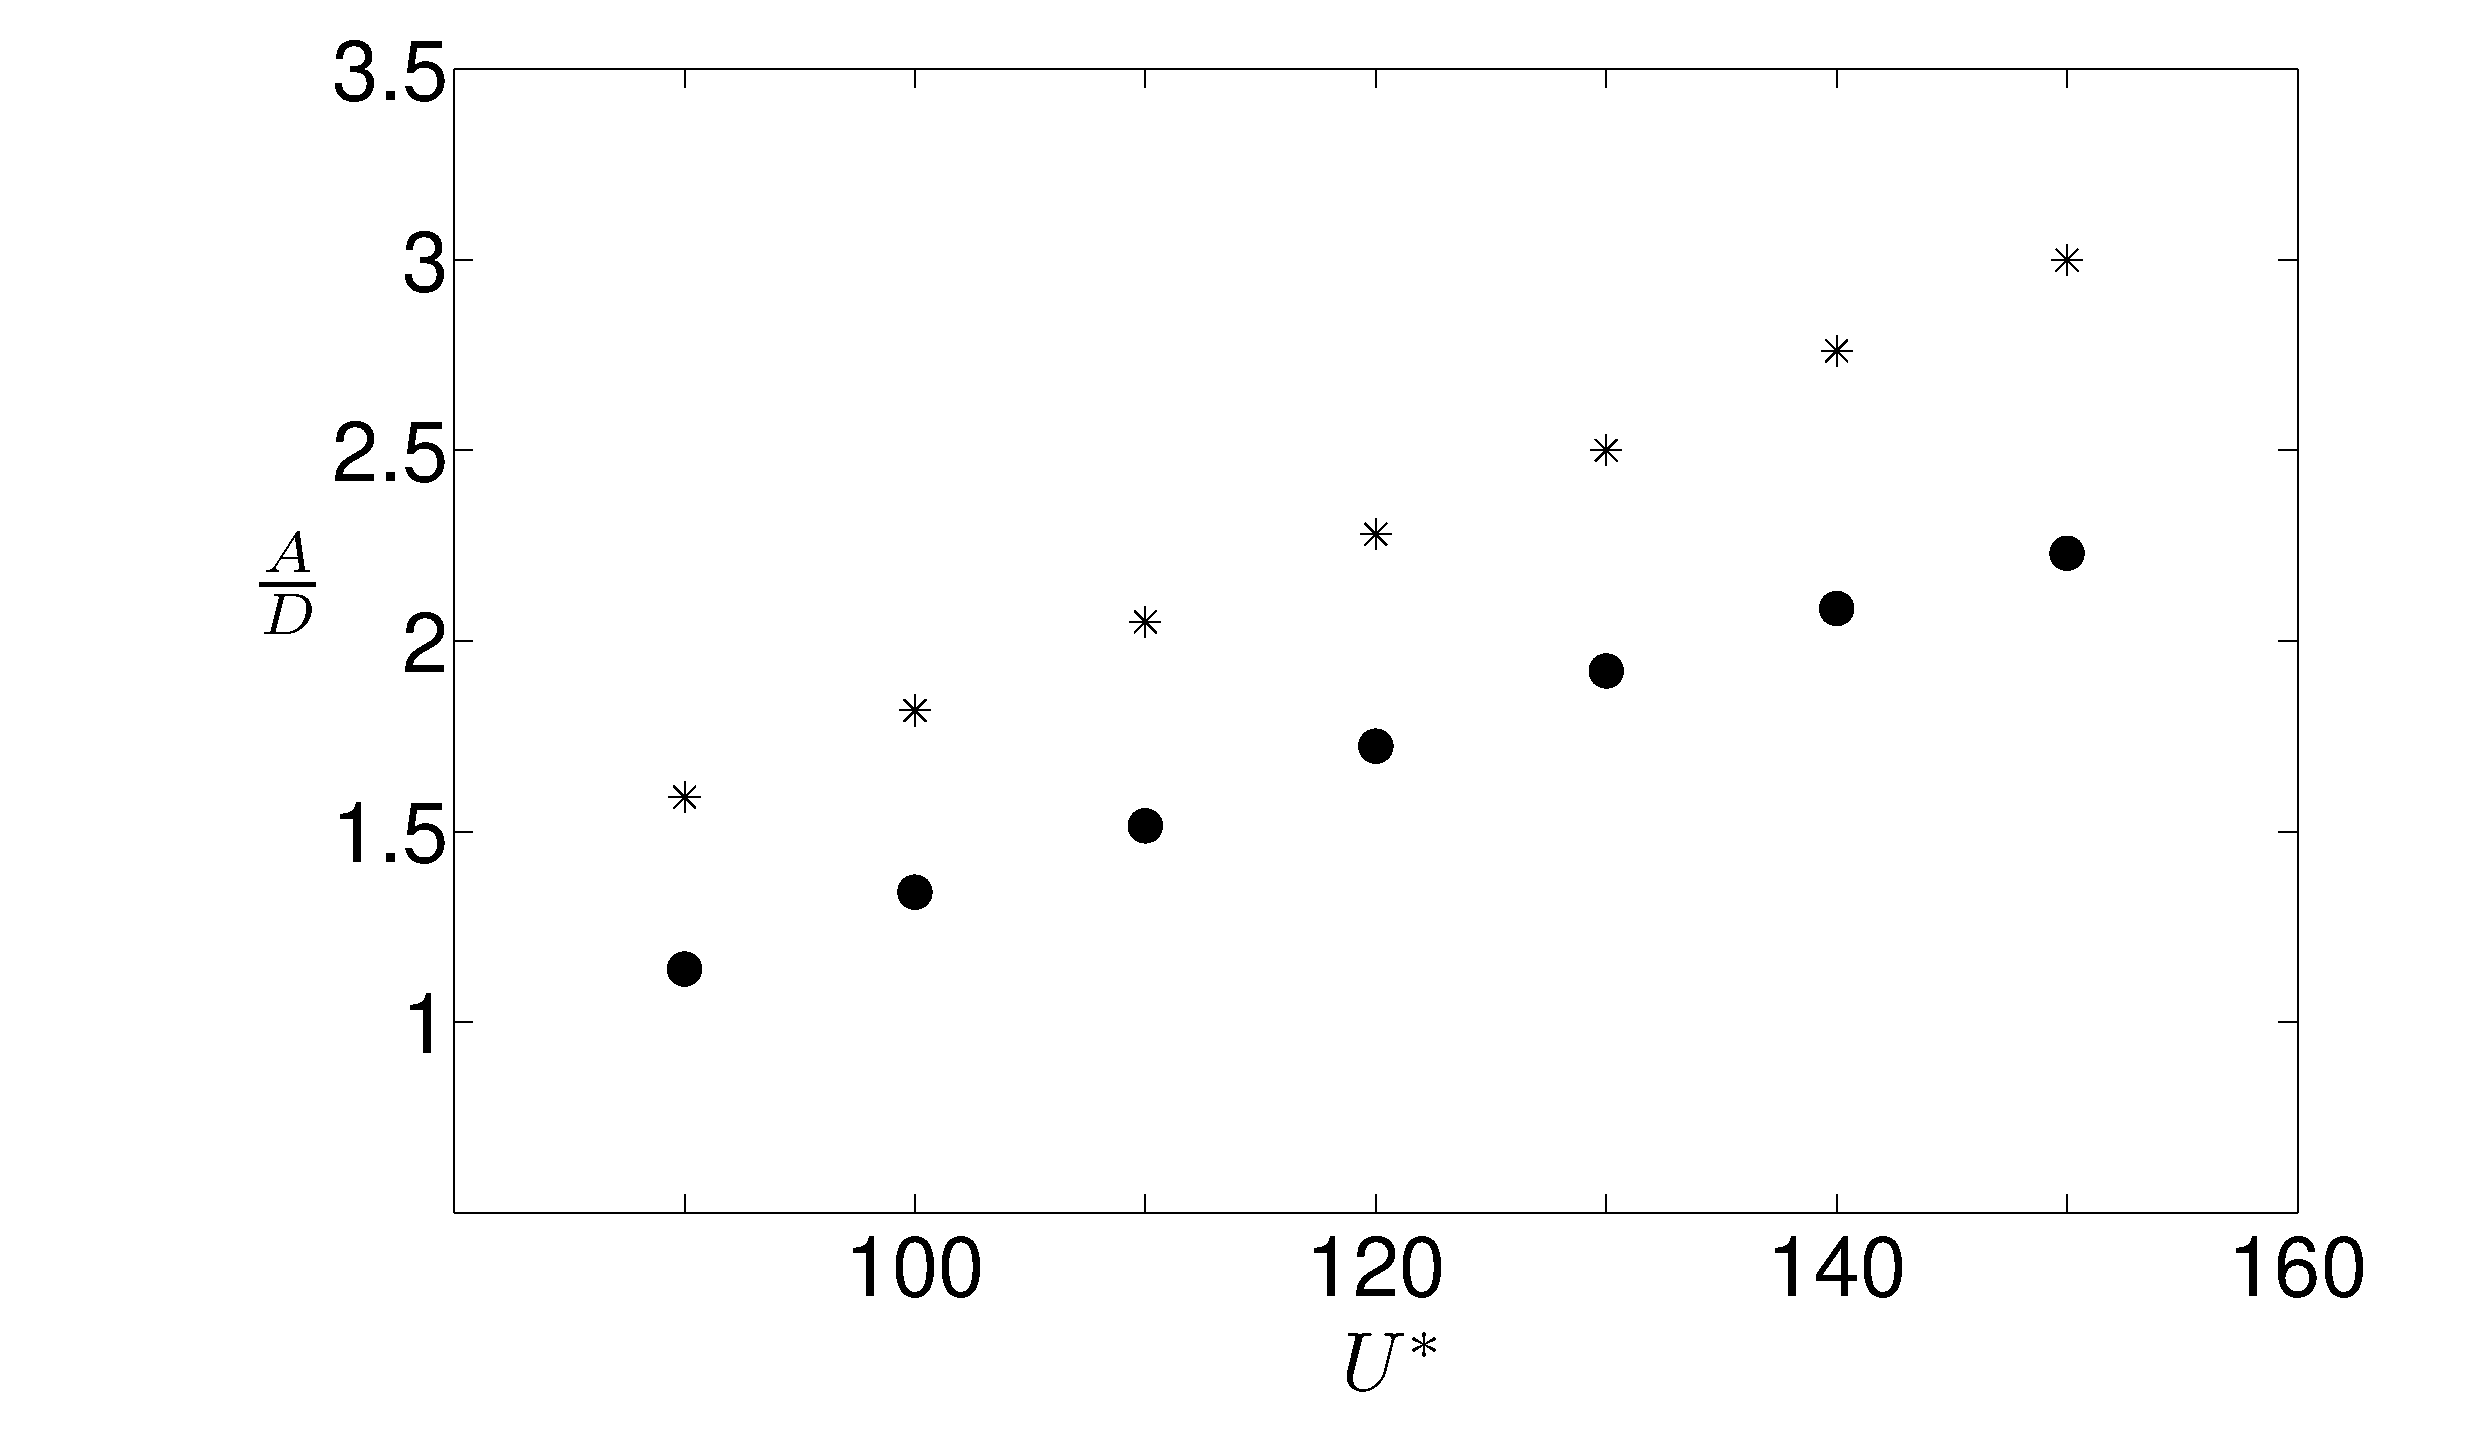
\includegraphics[width=0.8\linewidth]{../FnP/from_reynolds/QSS_FSI_dis_amp}
%\caption{QSS () and FSI data at Re 165 $\zeta=0.075$ $m^*=20$}
%\label{fig:QSS_FSI_dis_amp}
%\end{figure}

\begin{figure}
\centering
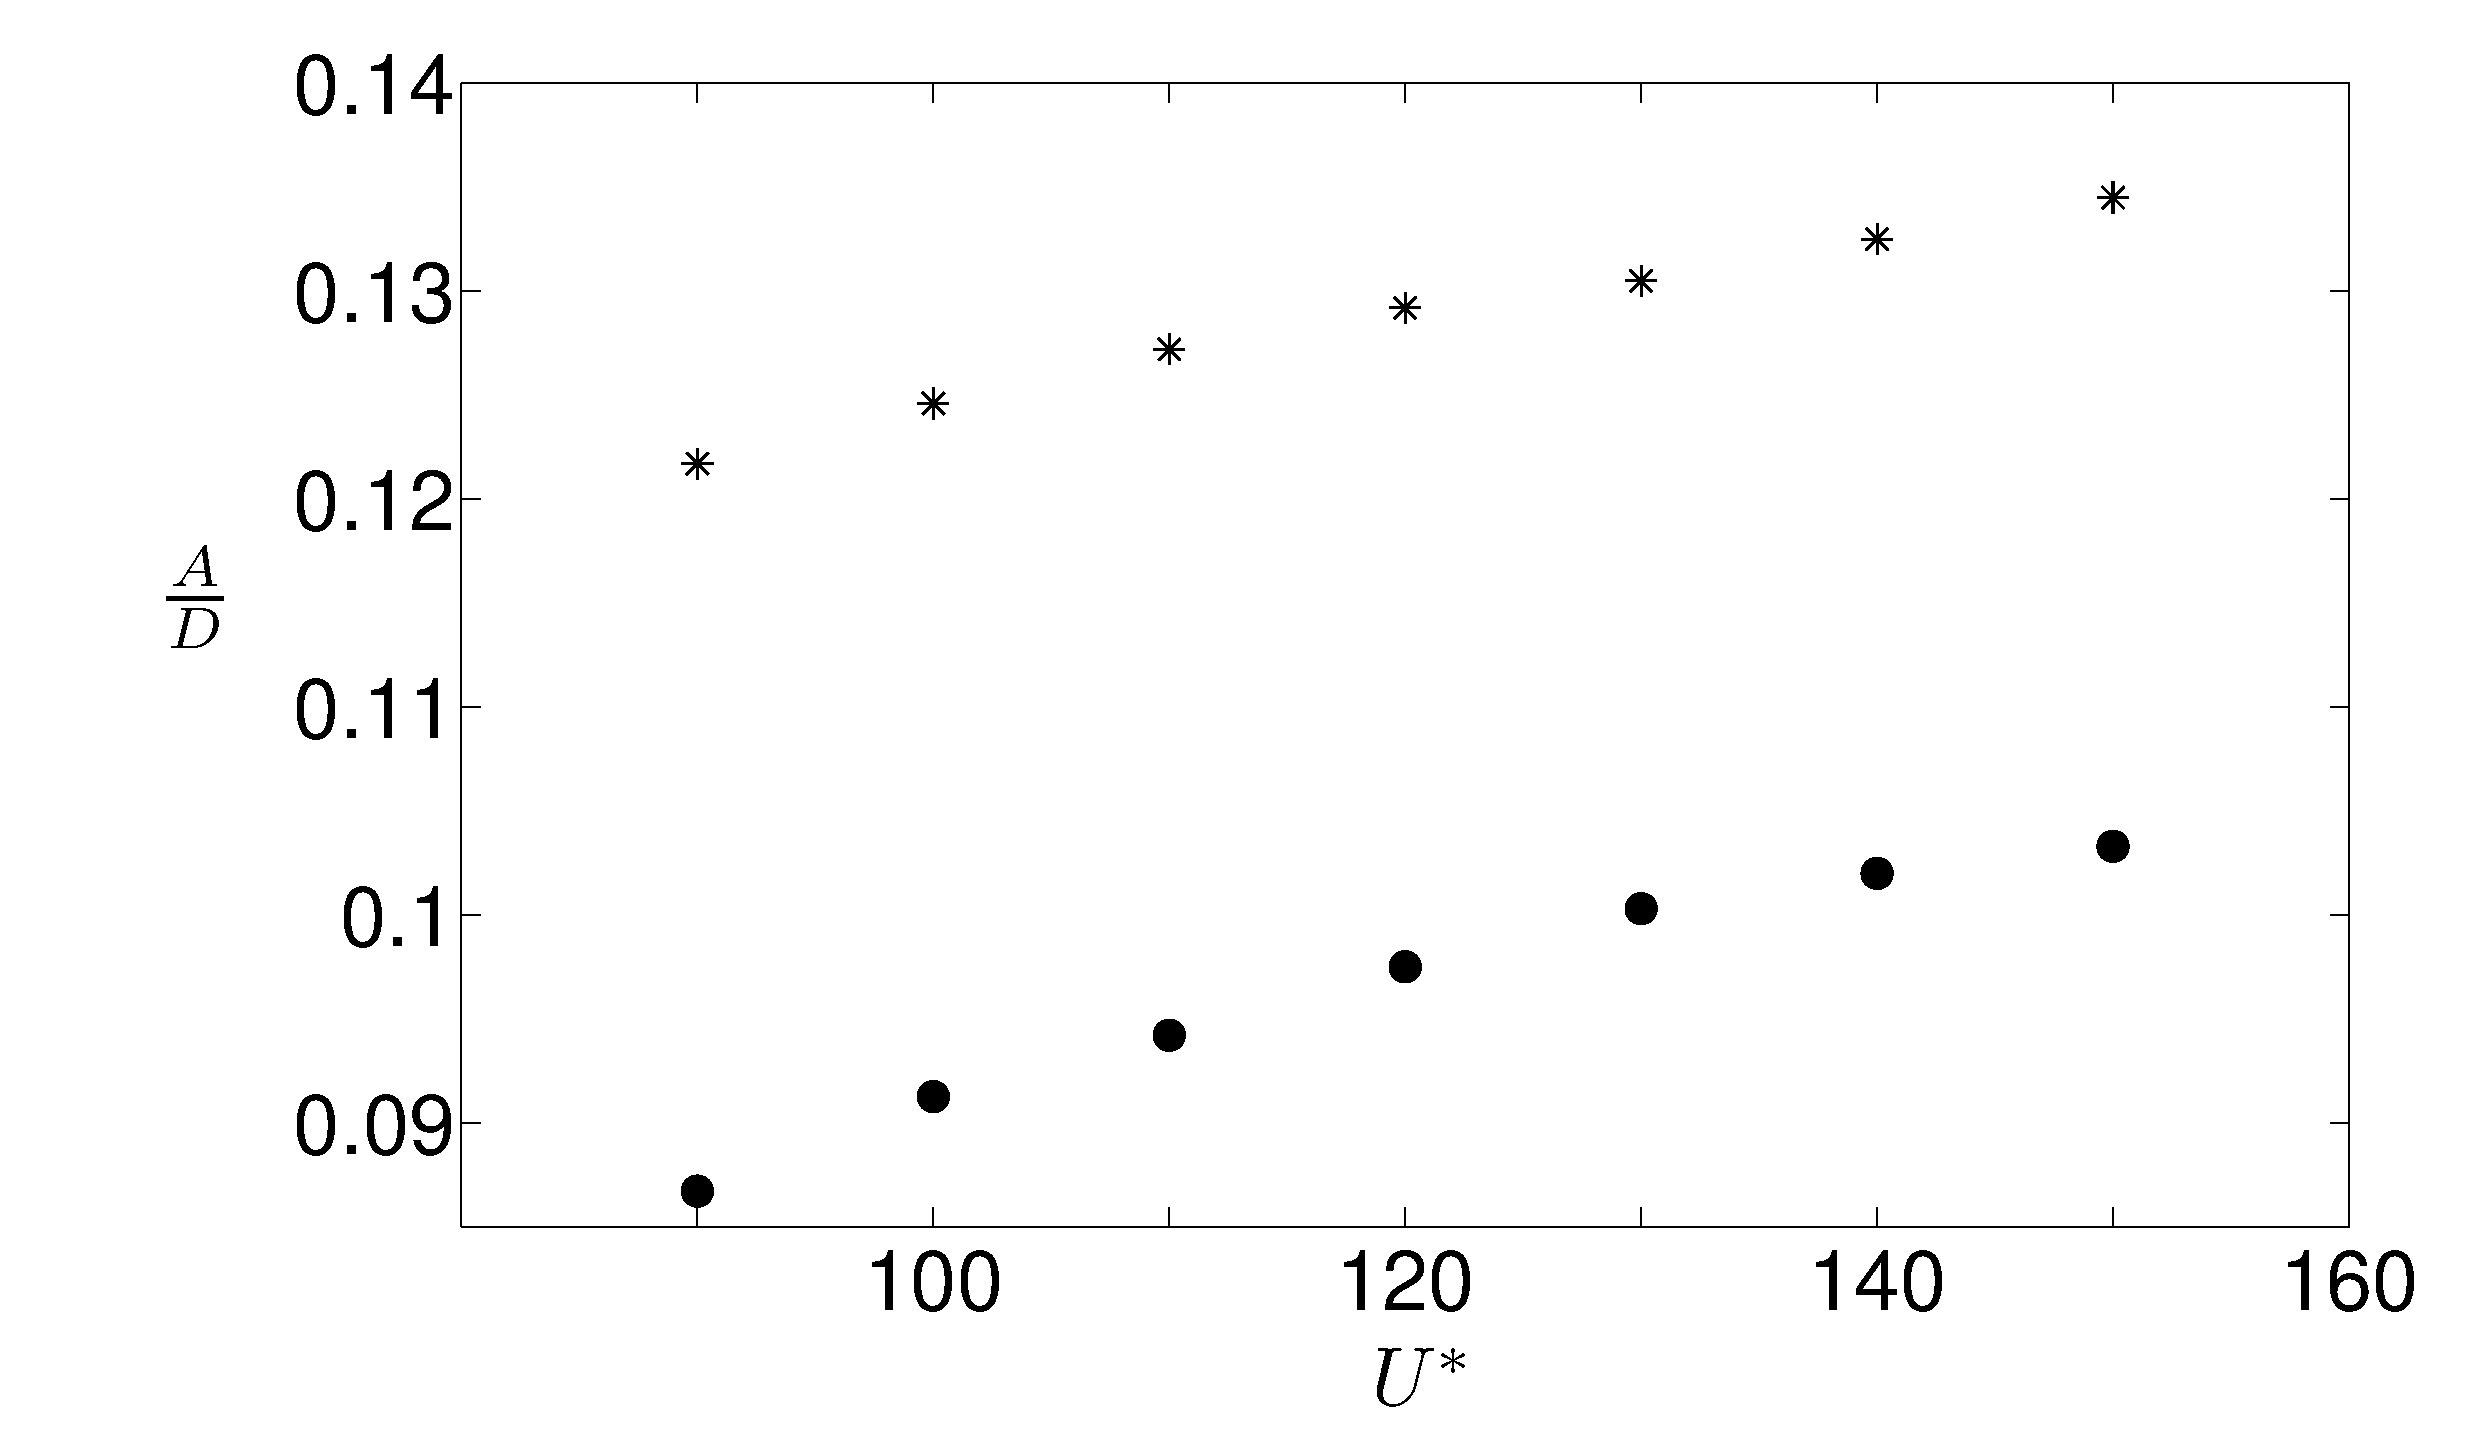
\includegraphics[width=0.8\linewidth]{../FnP/from_reynolds/QSS_FSI_vel_amp}
\caption{}
\label{fig:QSS_FSI_vel_amp}
\end{figure}



\section{Discussion}

$U^*$ and $\zeta$ has the natural frequency term inside it. Therefore when $U^*$ is varied keeping $\zeta$ constant the damping constant `$c$' varies is as well. The expression for `$c$' could be given from the following equation below

\begin{equation}
\label{equation_for_c}
c=\dfrac{4 \pi \zeta m^*}{U^*}
\end{equation}


Therefore if $m^*\zeta$ is kept constant (as done in \cite{Barrero-Gil2010a}) the damping constant `$c$' changes with $U^*$. According to the  equation of motion  Eq.\ref{final_equation_motion} the `$m$' and the `$k$' therms does not take out energy from the system and thereby `$c$' becomes the controlling parameter with regards to energy output. as from Eq.\ref{equation_for_c} we could see that $c\propto \dfrac{1}{U^*}$. As damping decreases with increasing $U^*$, the displacement and velocity amplitudes increases.

Power could be expressed as the product of force and velocity. Therefore the transferred power form fluid-to-body could be expressed as $P_t=F_y\dot{y}$. Similarly the dissipated power due to the mechanical damping could be expressed as $P_d=(c\dot{y})\dot{y}.$

The analysis of time histories of $P_t $ and $P_d$ at key regions on the mean power vs $U^*$ provides an detailed explanation on what exactly happens to power when the reduced velocity is increased. The 3 regions are illustrated in Fig. \ref{fig:sketch_1}. It should be noted that in order to obtained a clear signal the VIV is filtered out. The data are taken at $m^* = 40,\zeta=0.1,Re=165$ 

\begin{figure}
\centering
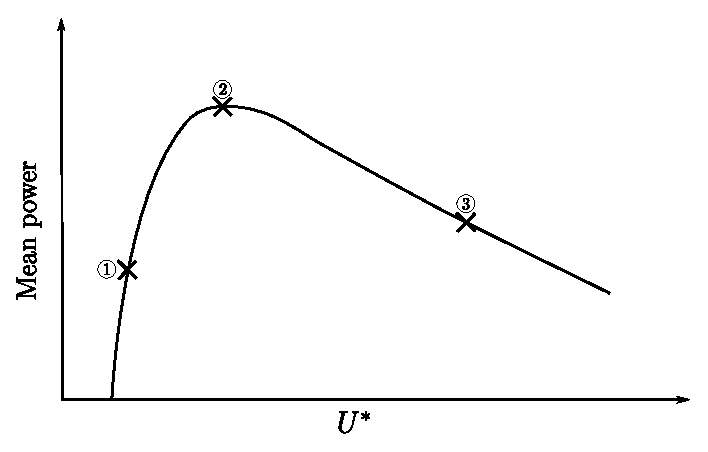
\includegraphics[scale=0.8]{../FnP/sketch_1}
\caption{}
\label{fig:sketch_1}
\end{figure}






\begin{figure}
\centering
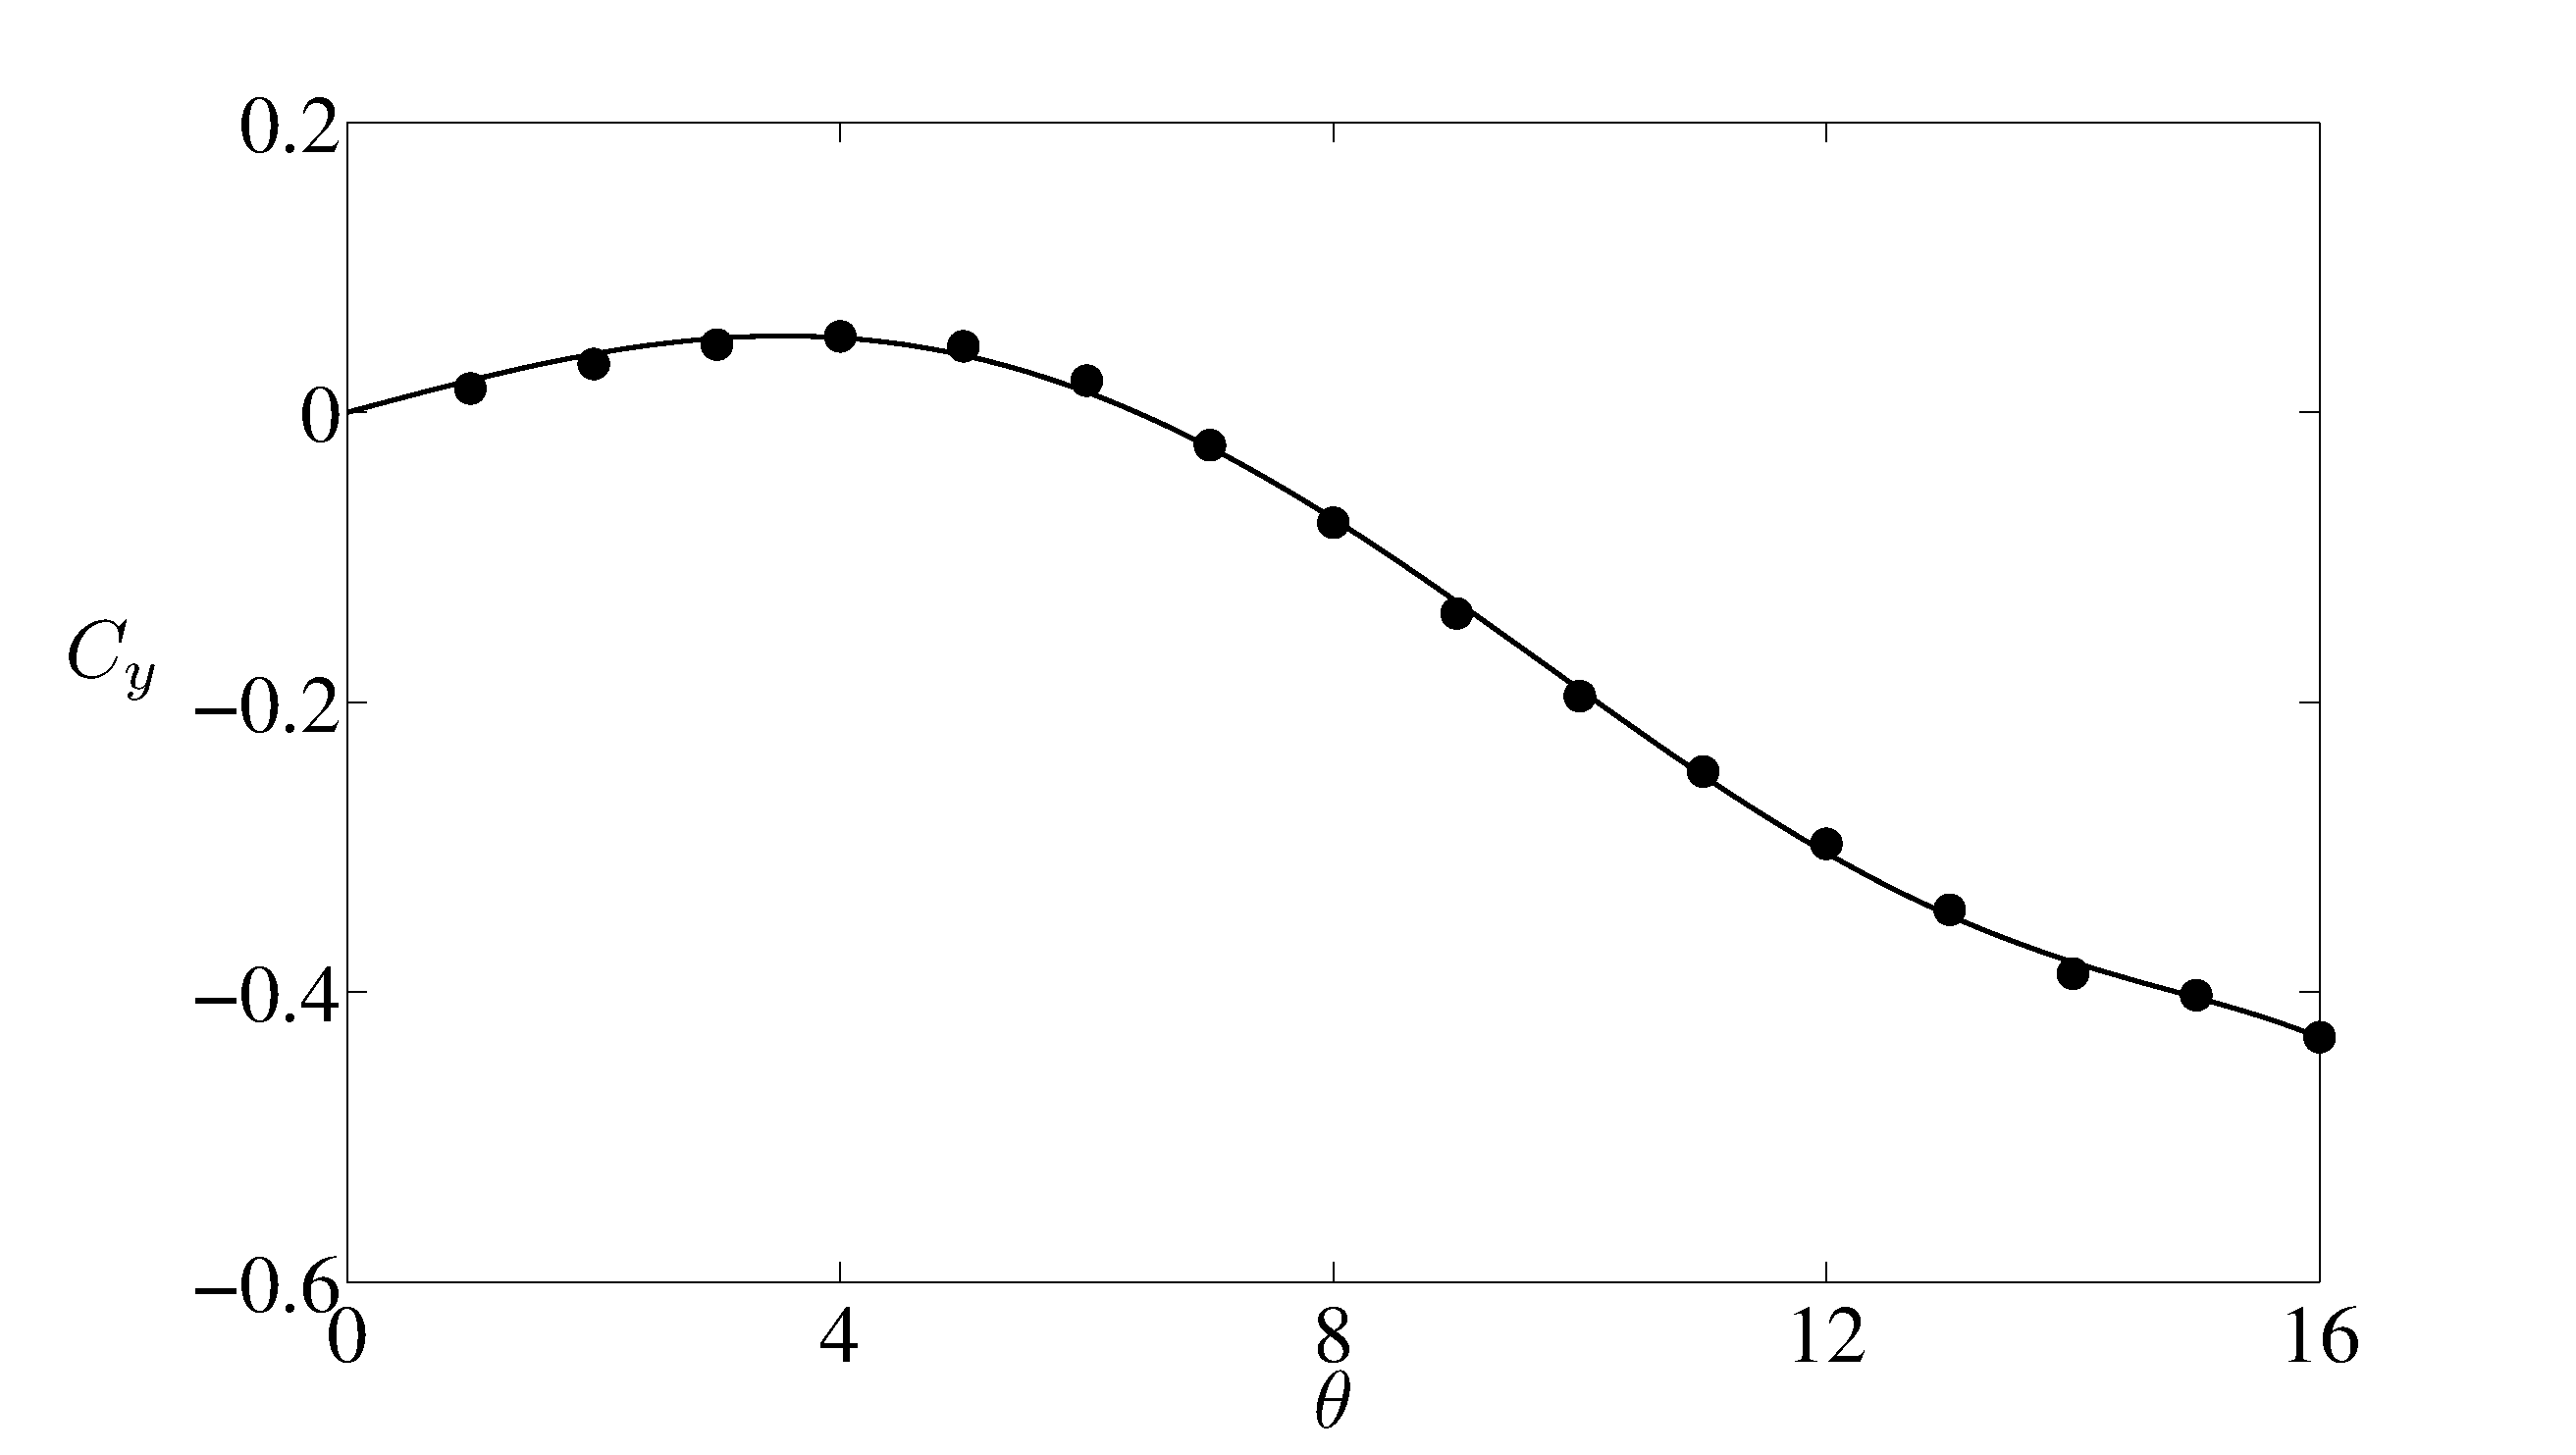
\includegraphics[width=0.8\linewidth]{../FnP/from_reynolds/lift_curve}
\caption{}
\label{fig:lift_curve}
\end{figure}


At  $U^*=90$ (region 1) the damping constant is high and therefore a clear sinusoidal signal could be observed for both $P_d$ and $P_t$ Fig. \ref{fig:power_time_hostory_u_90}. By Comparing time history of $\theta$ Fig. (\ref{fig:F_theta_history_u_90fig}) together with the $\theta$ vs. $C_y$ plot it is possible to see that the $\theta$  does not exceed the critical angle where the maximum $C_y$ (and therefore maximum $F_y$ )is produced. Hence both $P_d$ and $P_t$ becomes sinusoidal.
\begin{figure}
\centering
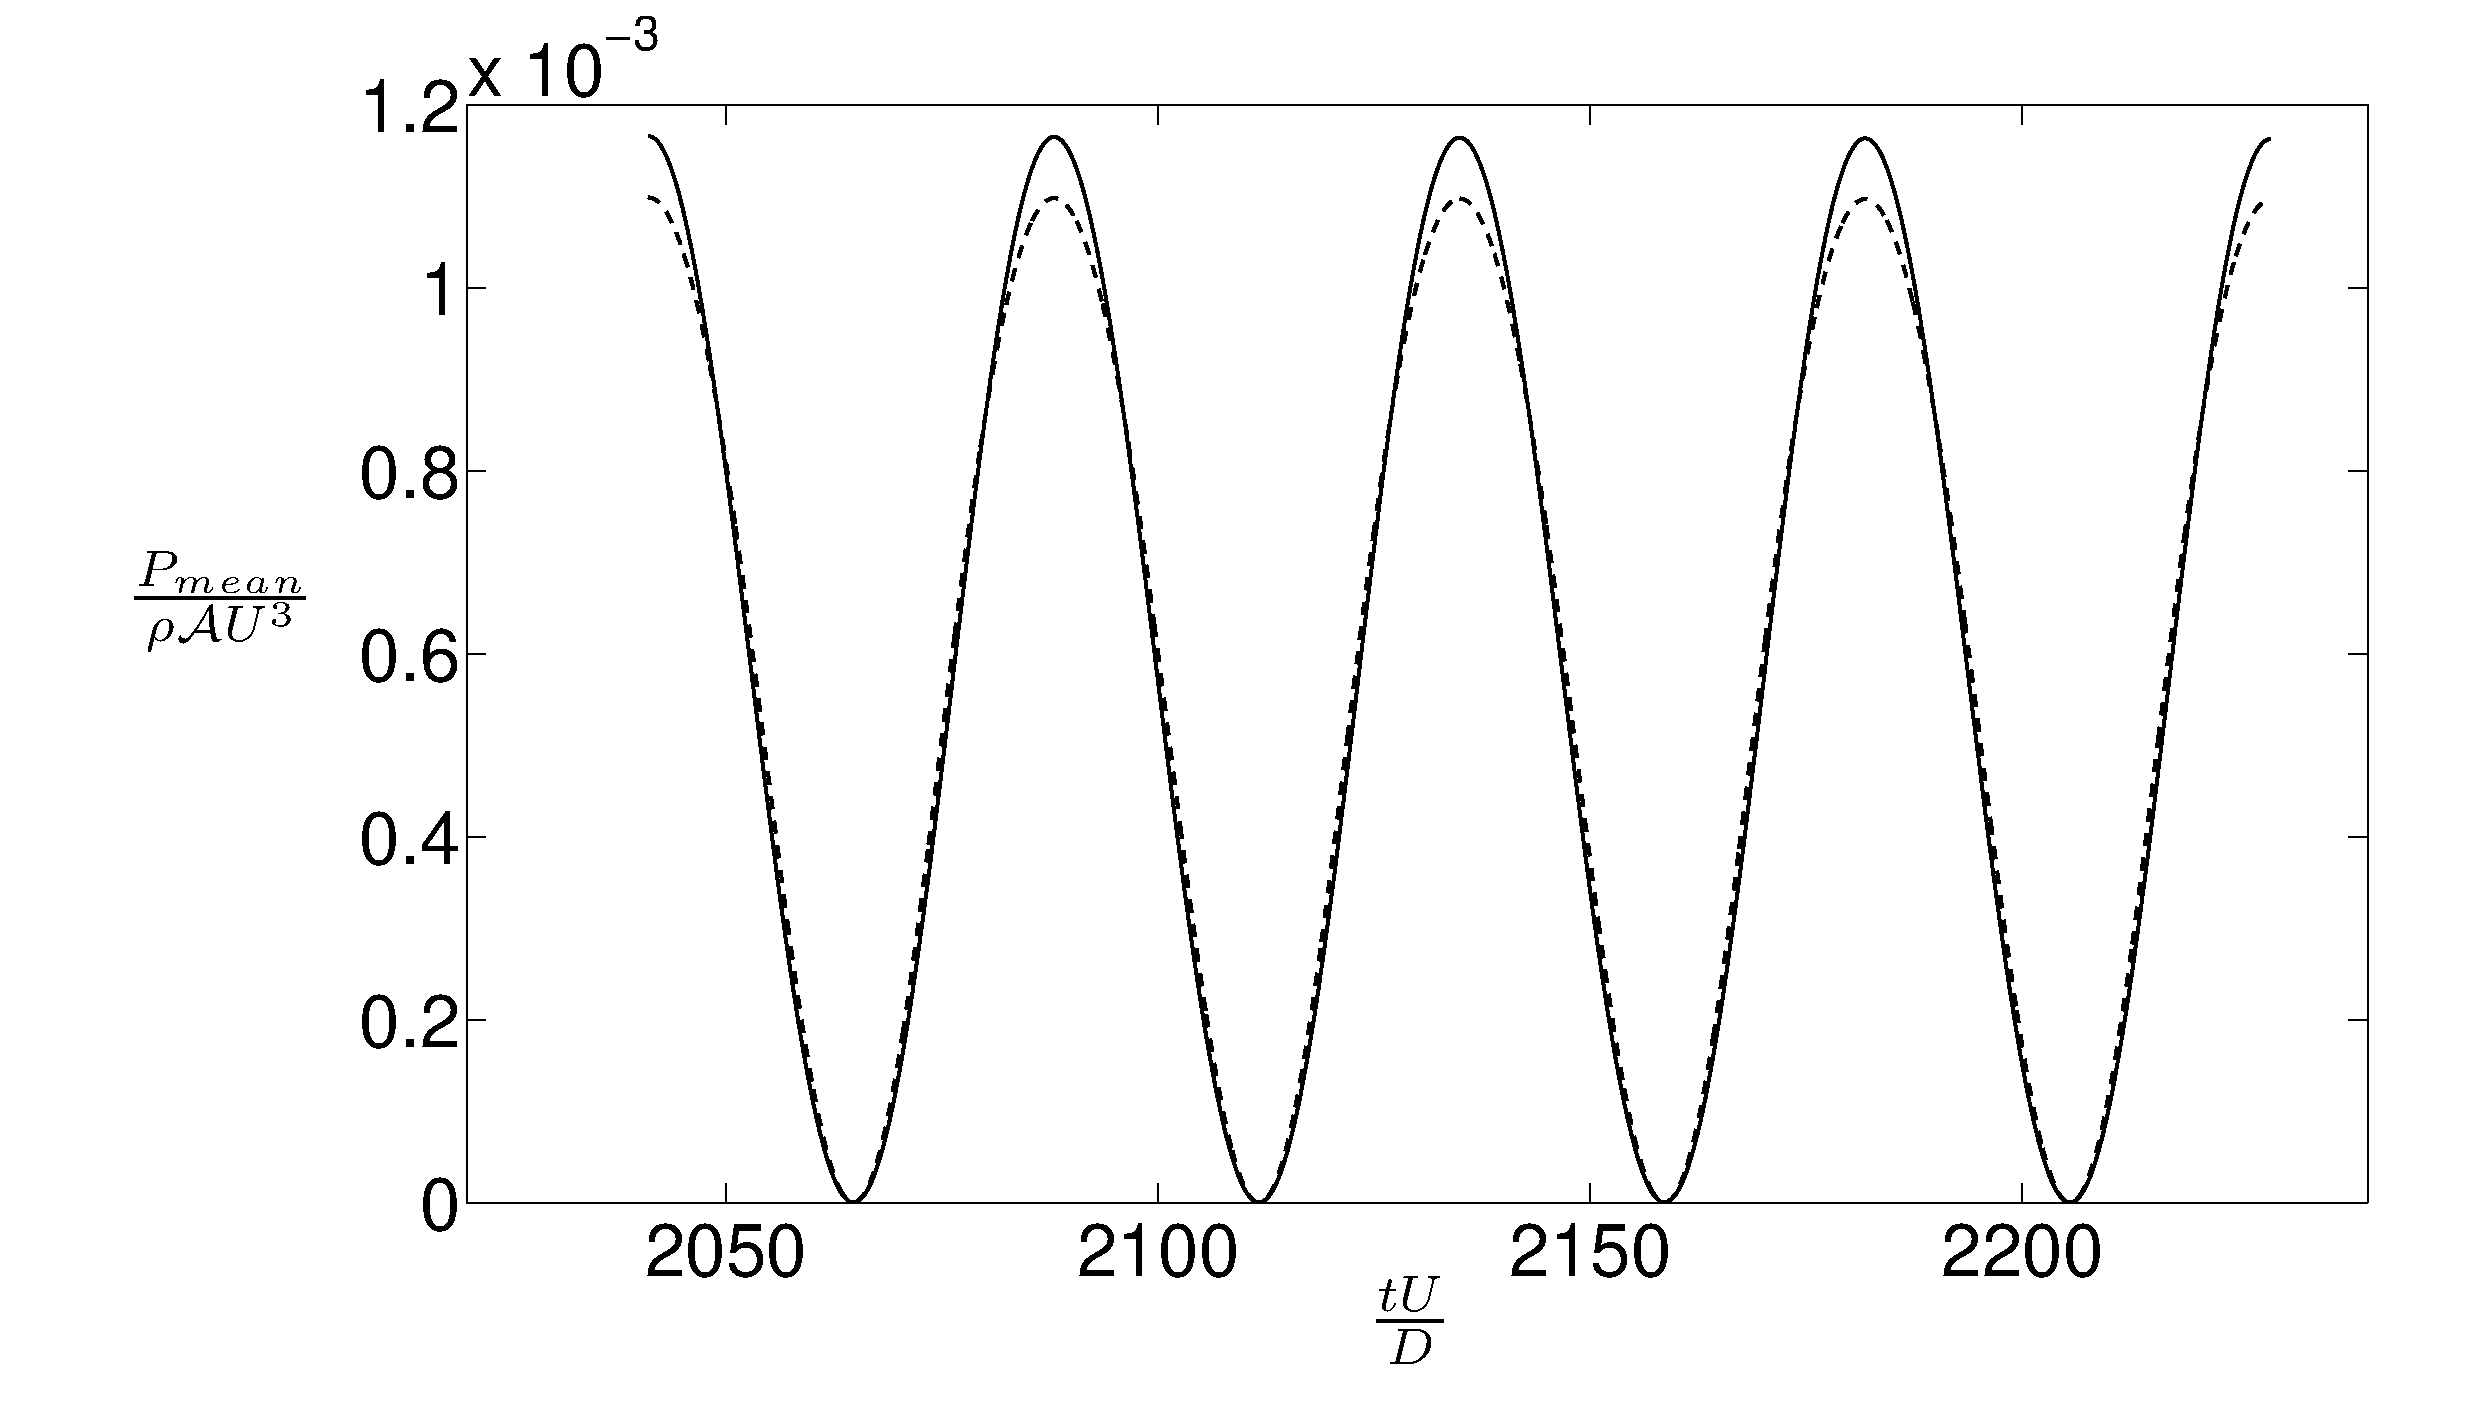
\includegraphics[width=0.8\linewidth]{../FnP/from_reynolds/power_time_hostory_u_90}
\caption{}
\label{fig:power_time_hostory_u_90}
\end{figure}

\begin{figure}
\centering
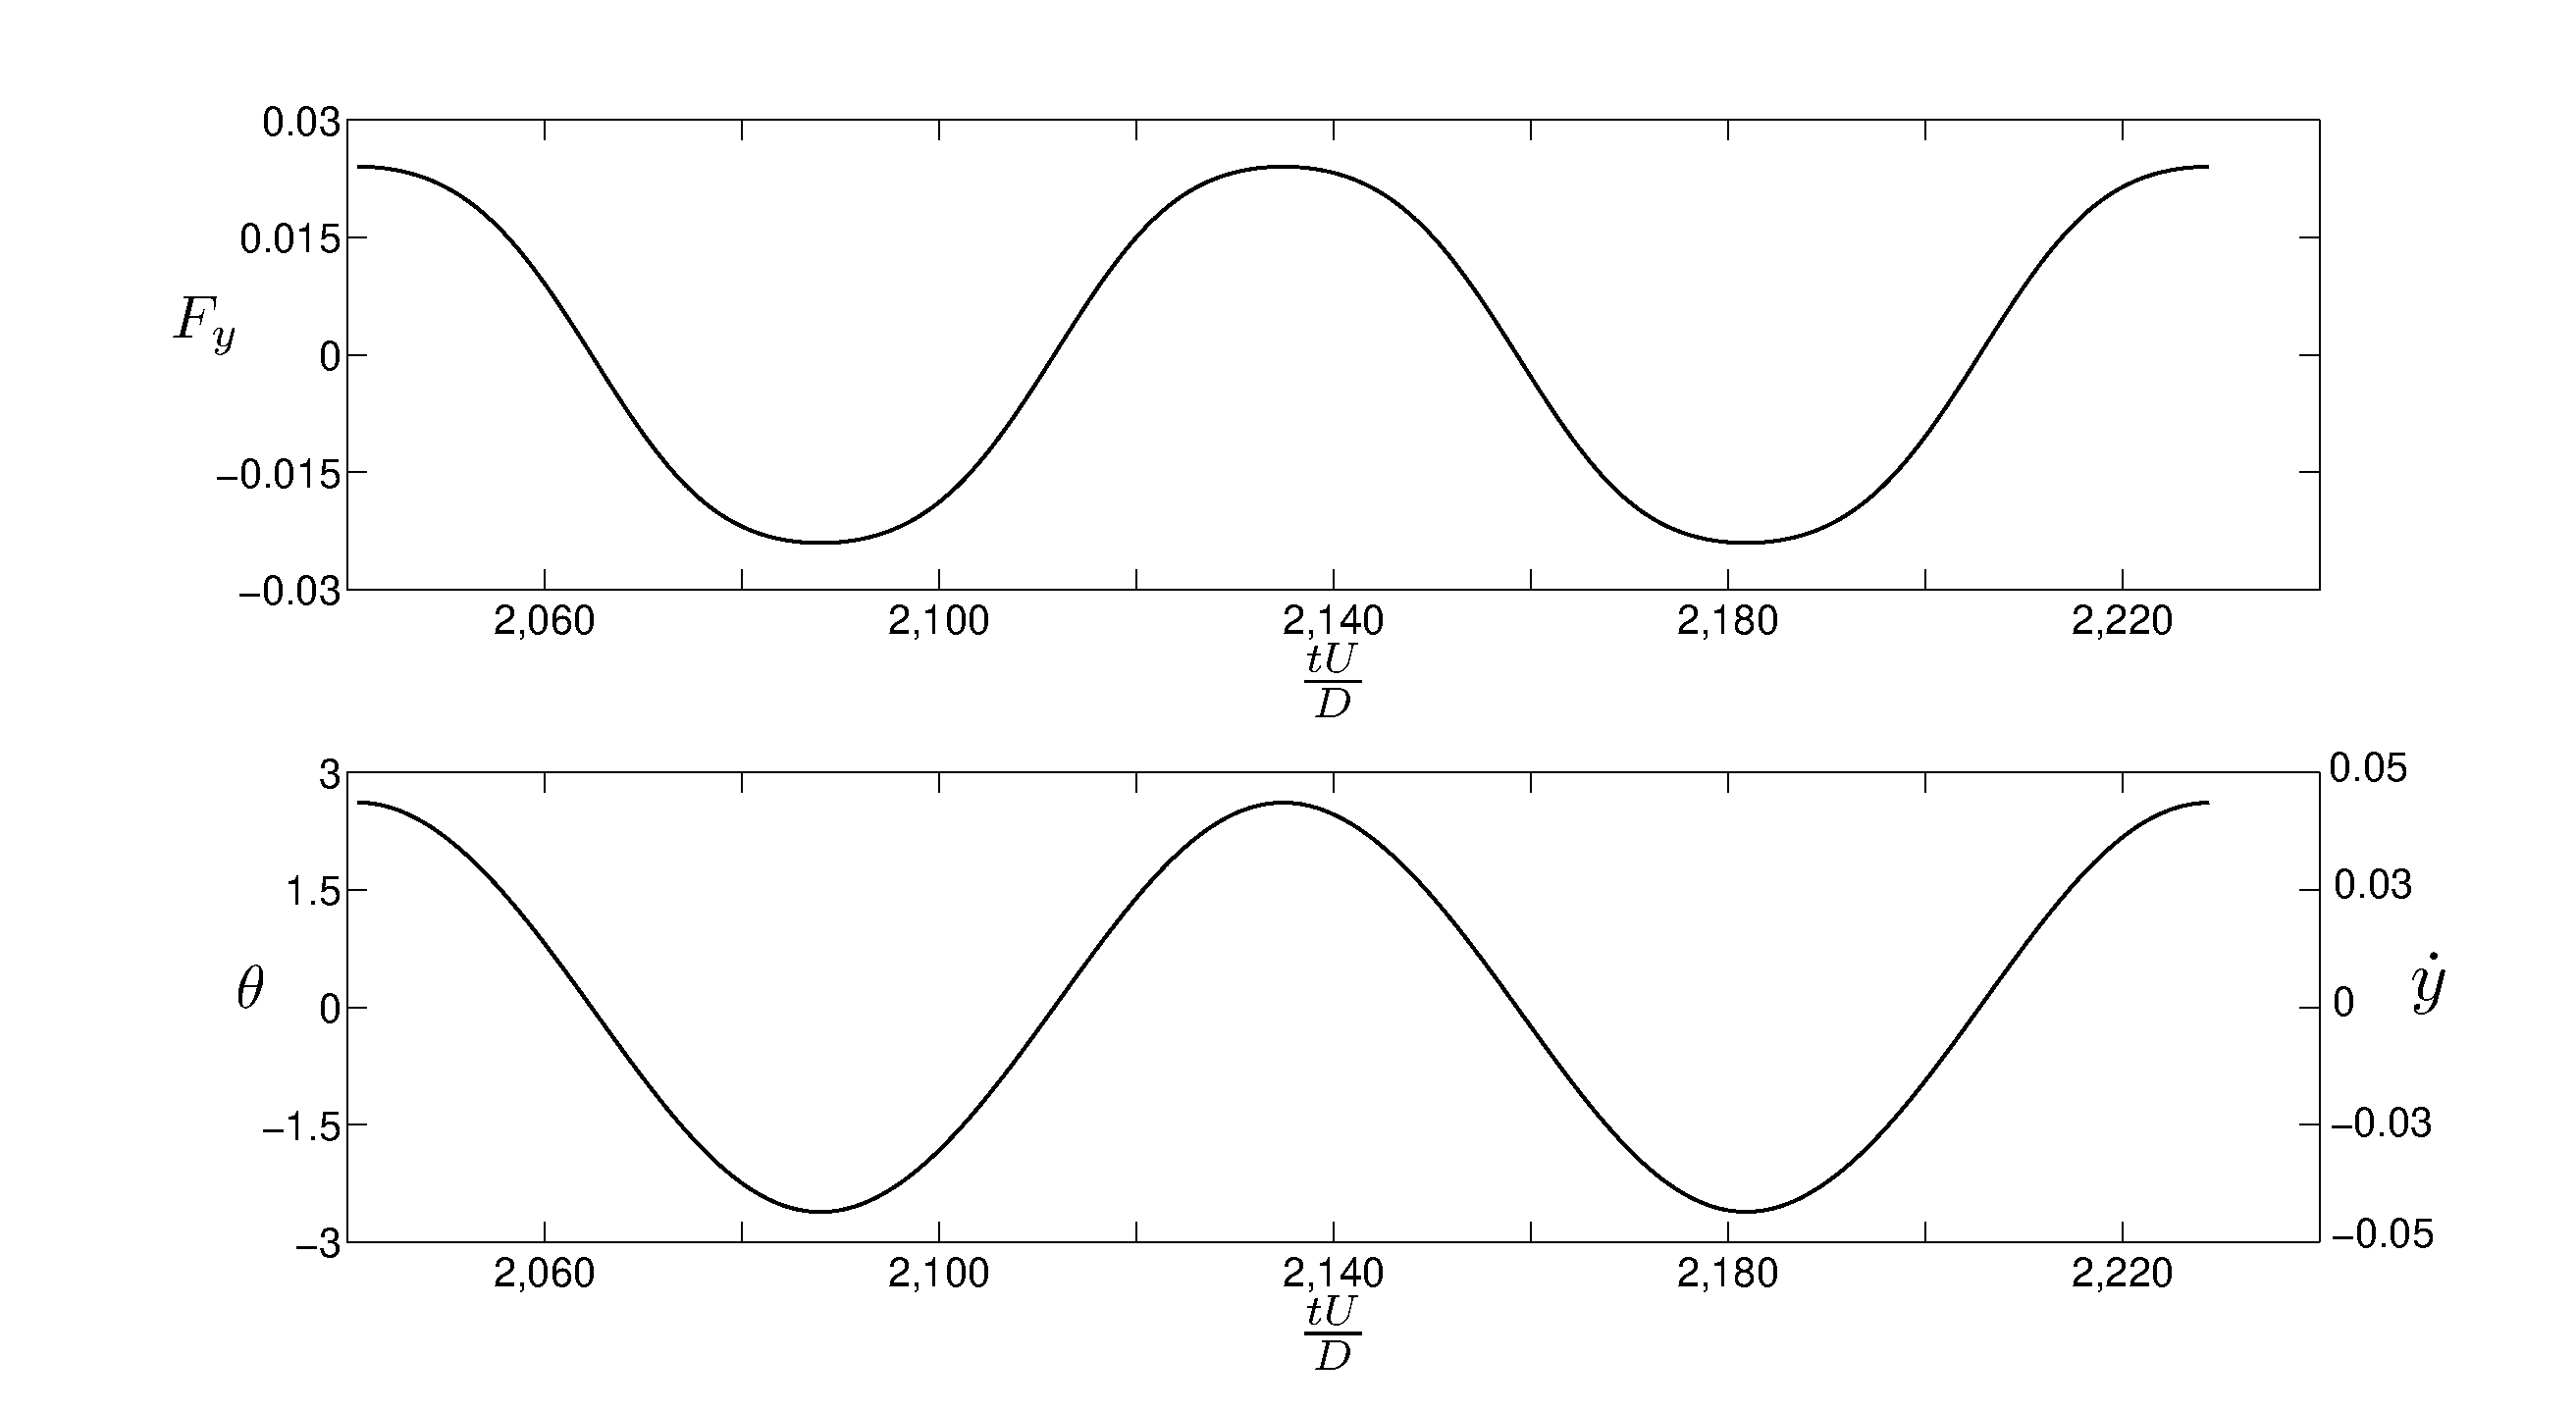
\includegraphics[width=1\linewidth]{../FnP/from_reynolds/F_theta_history_u_90fig}
\caption{}
\label{fig:F_theta_history_u_90fig}
\end{figure}



At region 2 ($U=165$) where the mean power becomes maximum, $P_t$ does not become a pure sinusoidal signal. However, the  signal remains periodic. From the time history graph of $P_t$ two `peaks' are present in a single half cycle (Fig \ref{fig:power_time_hostory_u_165}). Analysing  Fig. \ref{fig:F_theta_history_u_165} and \ref{fig:lift_curve} it could be observed that $\theta$ passes critical angle where the maximum $C_y$ is produced. Therefore, the force $F_y$ and $P_t$ reduces as the velocity increases. As the velocity $\dot{y}$ is sinusoidal $\theta$ recovers back and leading to two `peaks'  in a single half cycle.


\begin{figure}
\centering
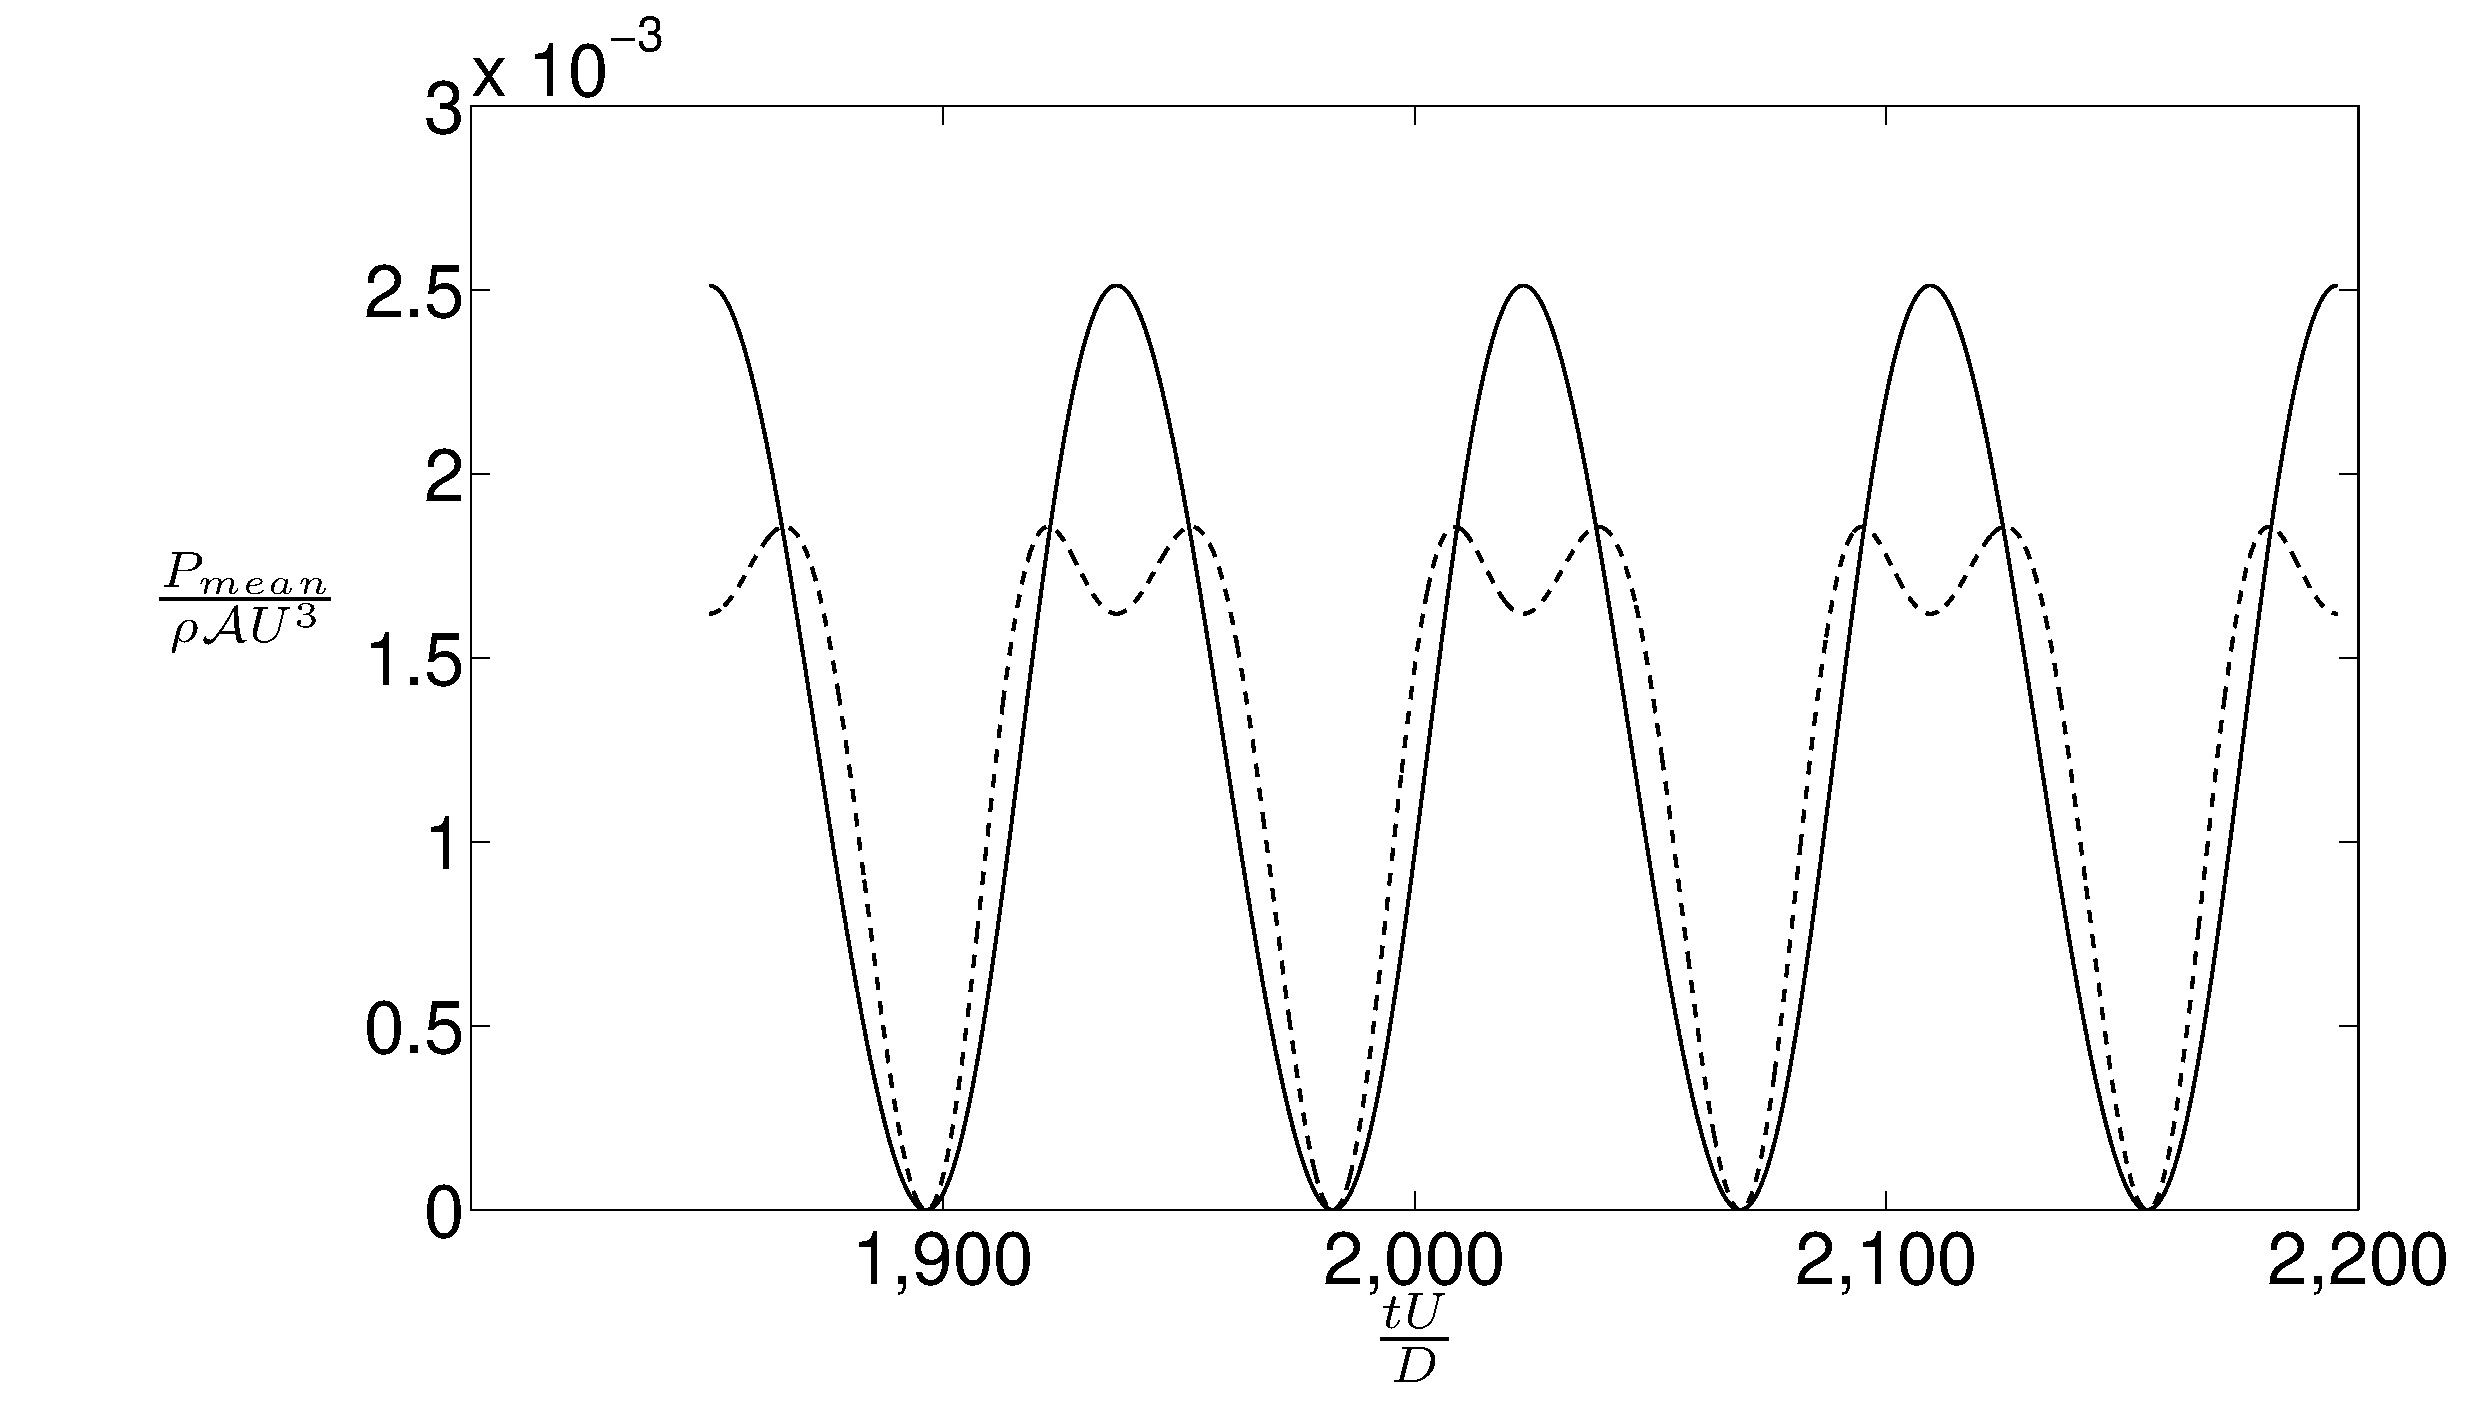
\includegraphics[width=0.8\linewidth]{../FnP/from_reynolds/power_time_hostory_u_165}
\caption{}
\label{fig:power_time_hostory_u_165}
\end{figure}

\begin{figure}
\centering
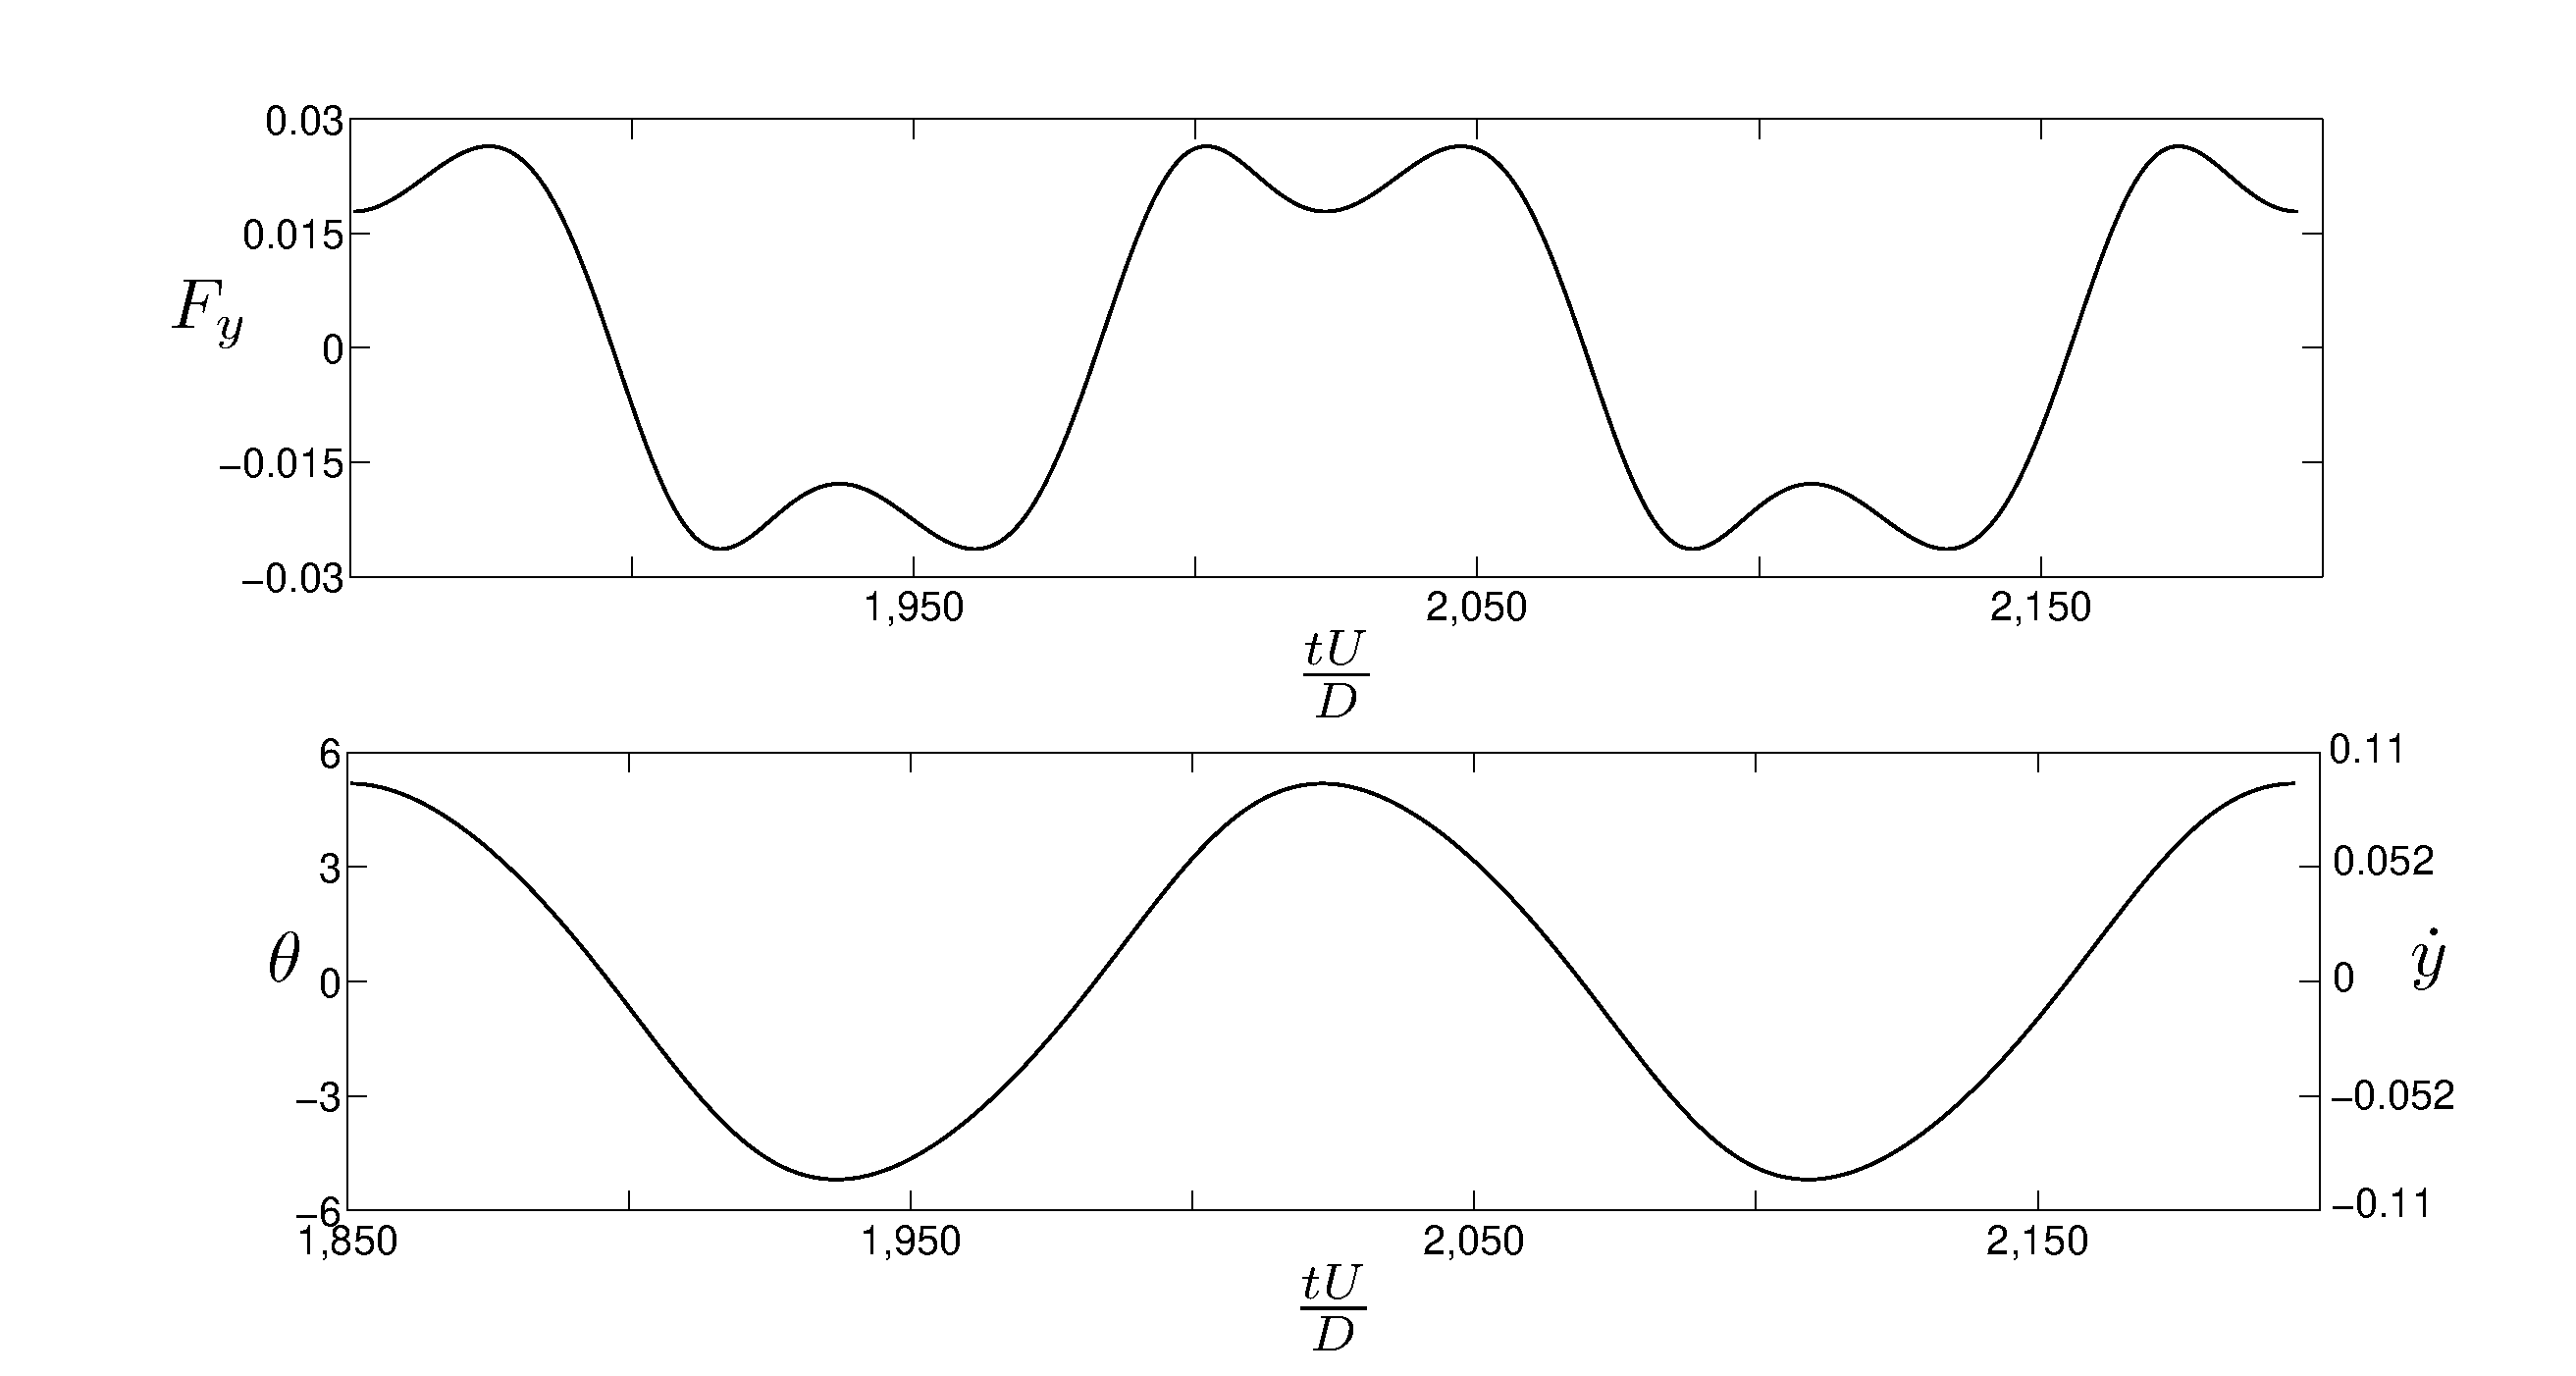
\includegraphics[width=1\linewidth]{../FnP/from_reynolds/F_theta_history_u_165}
\caption{}
\label{fig:F_theta_history_u_165}
\end{figure}


\begin{figure}
\centering
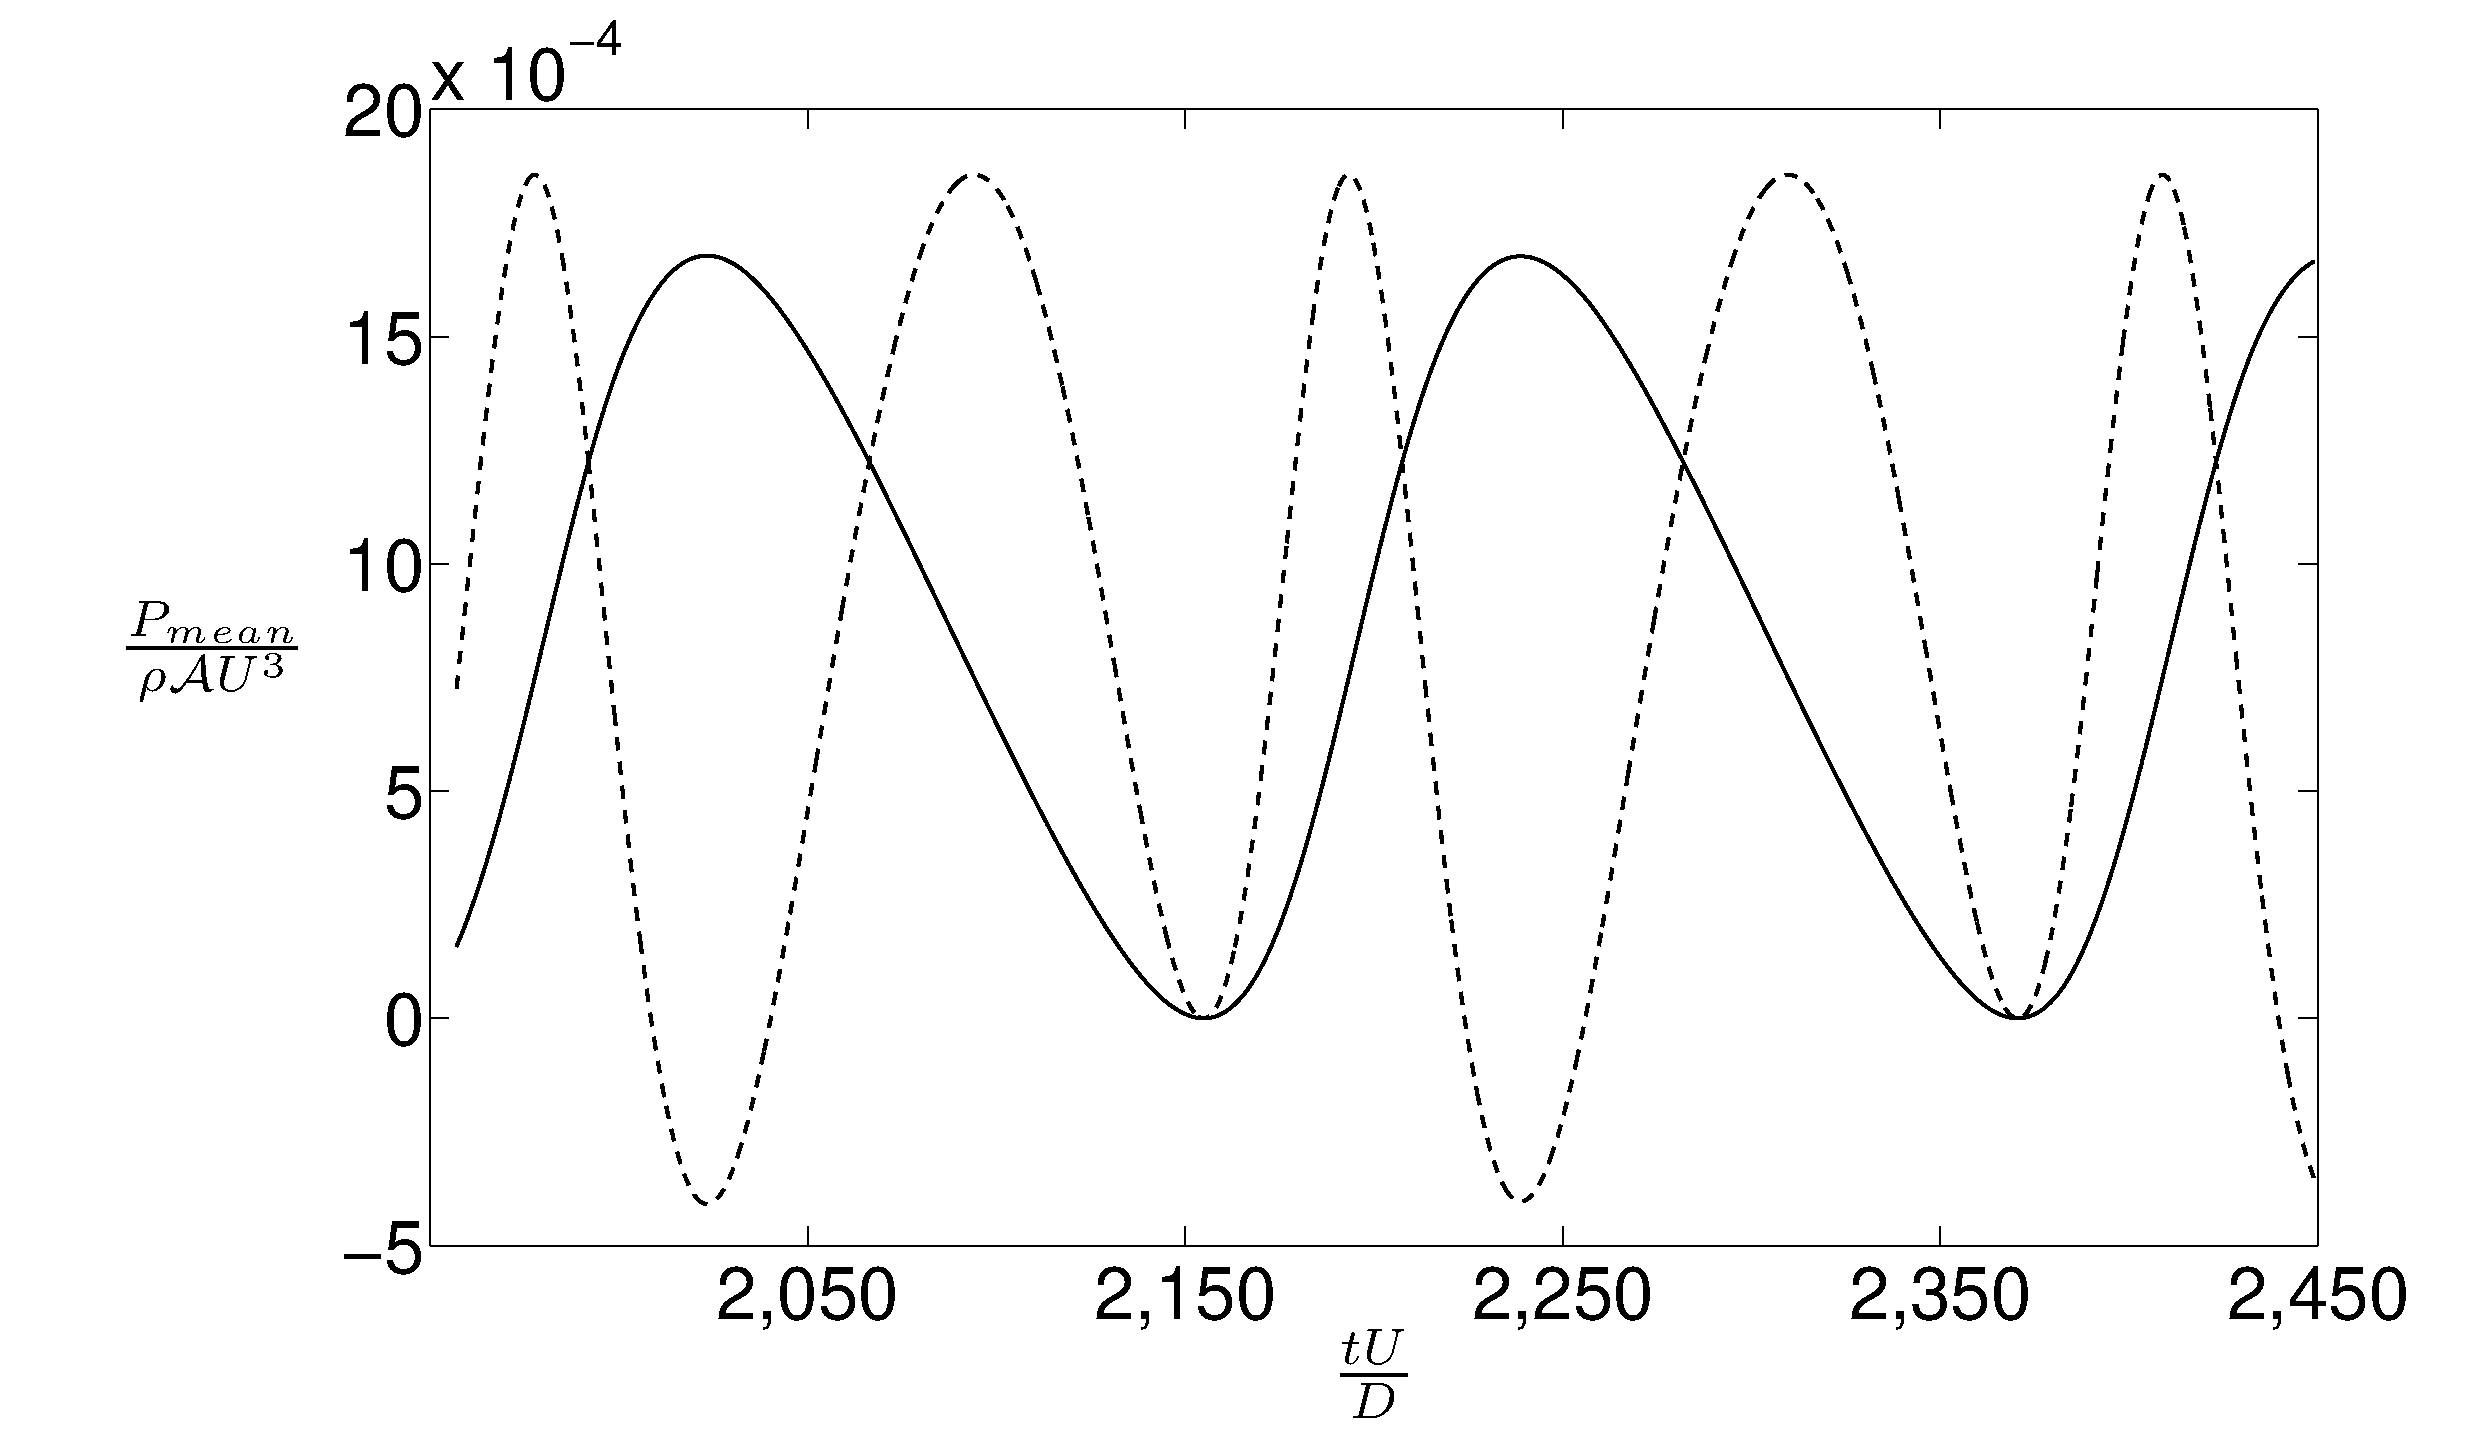
\includegraphics[width=0.8\linewidth]{../FnP/from_reynolds/power_time_hostory_u_400fig}
\caption{}
\label{fig:power_time_hostory_u_400fig}
\end{figure}

\begin{figure}
\centering
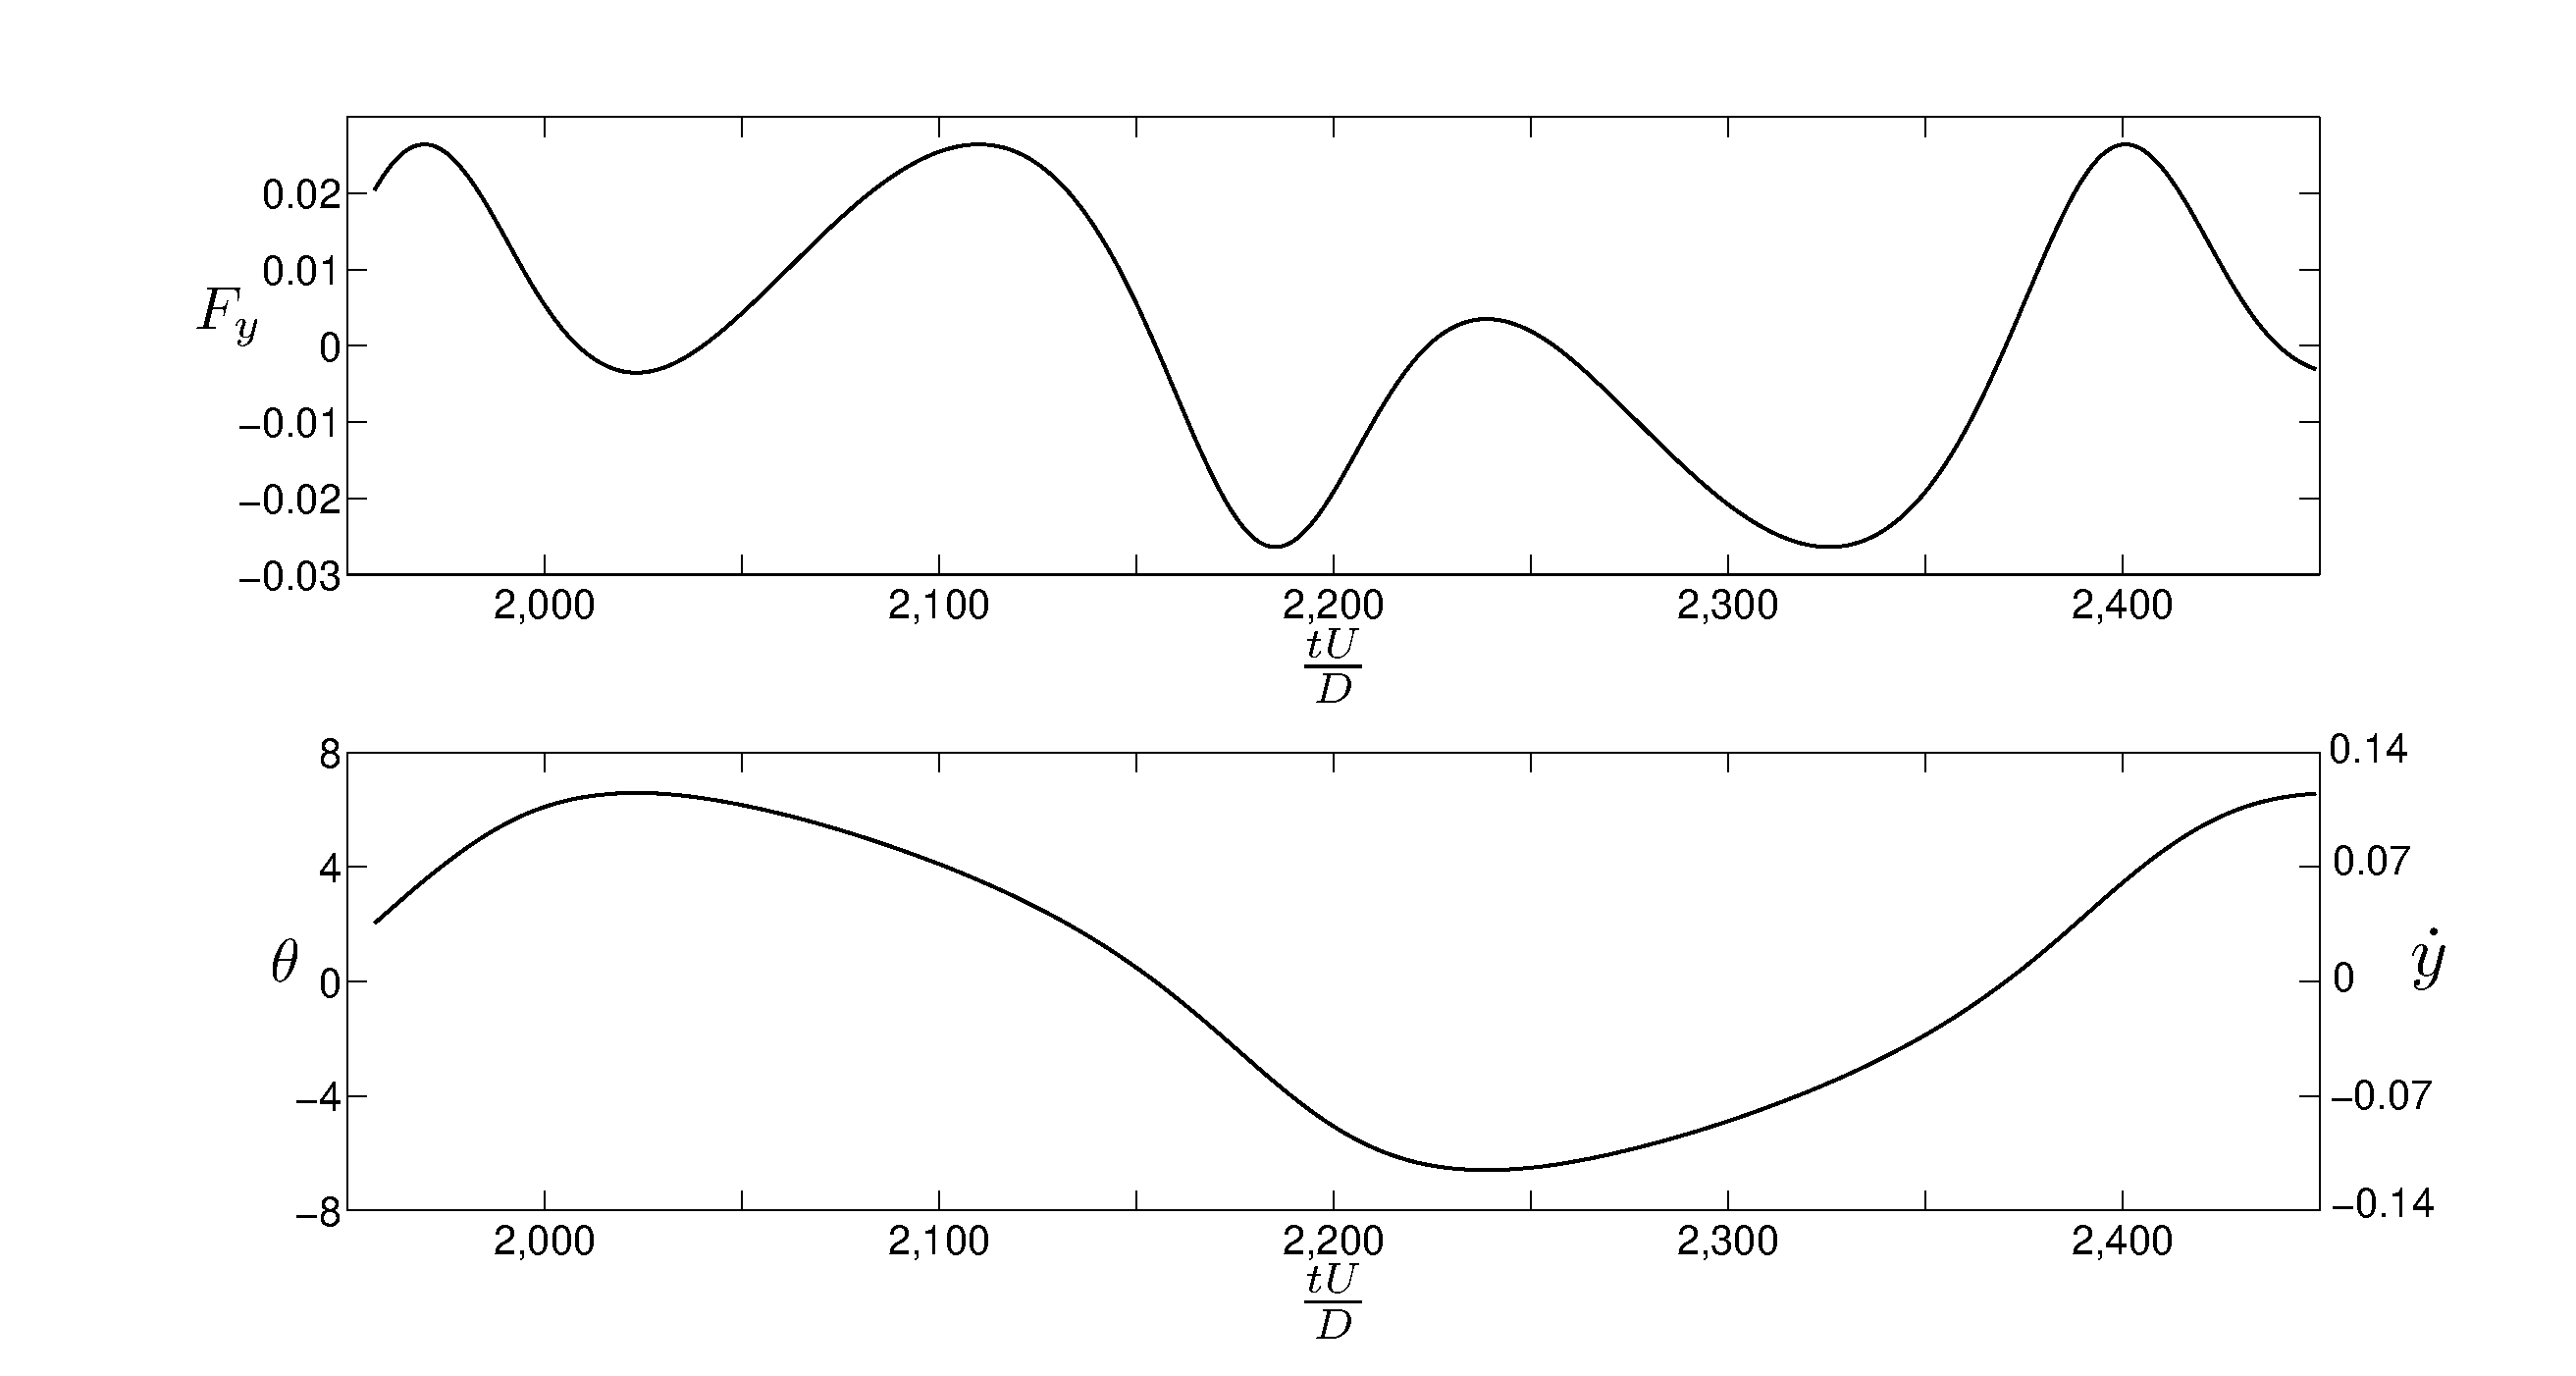
\includegraphics[width=1\linewidth]{../FnP/from_reynolds/F_theta_history_u_400}
\caption{}
\label{fig:F_theta_history_u_400}
\end{figure}


At region 3 ($U^*= 400$) `$c$' is significantly low therefore the mean power output is less. Furthermore by analysing the time history of $P_t$ and $P_d$ Fig. \ref{fig:power_time_hostory_u_400fig} it could be observed that $P_t$ becomes negative. This is due to the fact that $\theta$ moves to a region where $F_y$ becomes negative while velocity is positive. Hence $P_t$ becomes positive. On the other hand in therms of an energy point  of view, the mechanical damping is not sufficient to dissipate out the total transferred energy (as 1`'$C$' is substantially low), therefore  part of it  is transferred back to the fluid. 


As a summary it is possible to see that the rise and fall of the mean power occur due to change in `$c$' with $U^*$ eventhough $\zeta$ is kept constant. Therefore it is justifiable to say that a better way of representation of mean power is as a function of `$c$' rather than $U^*$. Furthermore we could see that the  unlike in VIV where $U^*$ plays a major role in achieving synchronisation, in galloping the tuning parameter of the mechanical system to optimise the mean power output is the damping constant `$c$' and not $U^*$ or any other parameter in the mechanical system.







